%%%%%%%%%%%%%%%%%%%%%%%%%%%%%%%%%%%%%%%%%%%%%%%%%%%%%%%
%% Bachelor's & Master's Thesis Template             %%
%% Copyleft by Artur M. Brodzki & Piotr Woźniak      %%
%% Faculty of Electronics and Information Technology %%
%% Warsaw University of Technology, 2019-2020        %%
%%%%%%%%%%%%%%%%%%%%%%%%%%%%%%%%%%%%%%%%%%%%%%%%%%%%%%%

\documentclass[
    left=2.5cm,         % Sadly, generic margin parameter
    right=2.5cm,        % doesnt't work, as it is
    top=2.5cm,          % superseded by more specific
    bottom=3cm,         % left...bottom parameters.
    bindingoffset=6mm,  % Optional binding offset.
    nohyphenation=false % You may turn off hyphenation, if don't like.
]{eiti/eiti-thesis}

\langpol % Dla języka angielskiego mamy \langeng
\usepackage{microtype}   % Protrusion i expansion — zmniejsza overfull hboxy
\usepackage{xurl}        % Pozwala \url{} łamać linię w dowolnym miejscu (/, -, .)
\usepackage{seqsplit}    % Łamanie długich ciągów bez spacji (np. nazwy plików w \texttt{})
\usepackage{subcaption}  % Subfigures z podpisami (a), (b)
\usepackage{dirtree}     % Drzewa katalogów
\usepackage{float}       % Wymuszanie pozycji figur przez [H]
\usepackage{wrapfig}     % Tekst opływający grafikę
\usepackage{tikz}
\usetikzlibrary{shapes.geometric, arrows.meta, positioning, calc}
\graphicspath{{img/}}    % Katalog z obrazkami.
\addbibresource{bibliografia.bib} % Plik .bib z bibliografią

% ---- Konfiguracja listingów kodu ----
\lstdefinelanguage{Kotlin}{
    keywords={fun, val, var, if, else, for, while, return, object, class,
               interface, when, in, out, is, as, true, false, null, this,
               super, override, private, public, internal, protected,
               companion, data, sealed, abstract, open, by, get, set,
               import, package, throw, try, catch, finally, continue, break},
    morestring=[b]",
    morestring=[b]',
    morecomment=[l]{//},
    morecomment=[s]{/*}{*/},
    sensitive=true
}
\lstset{
    language=Kotlin,
    basicstyle=\small\ttfamily,
    keywordstyle=\bfseries,
    commentstyle=\itshape,
    stringstyle=\ttfamily,
    numbers=left,
    numberstyle=\scriptsize,
    numbersep=8pt,
    breaklines=true,
    captionpos=b,
    frame=single,
    framesep=4pt,
    xleftmargin=1.5em,
    tabsize=4,
    showstringspaces=false
}

\begin{document}

%--------------------------------------
% Strona tytułowa
%--------------------------------------
\EngineerThesis
\instytut{Telekomunikacji i Cyberbezpieczeństwa}
\kierunek{Telekomiunikacja}
\specjalnosc{Techniki Teleinformatyczne}
\title{
Monitorowanie położenia zwierząt z geofencingiem w sieci mesh LoRa}
\engtitle{
    Animal position monitoring with geofencing in a LoRa mesh network

}
\author{Józef Sławiński}
\album{278271}
\promotor{mgr. inż.\ Marcin Golański}
\date{\the\year}
\maketitle

%--------------------------------------
% Streszczenie po polsku
%--------------------------------------
\cleardoublepage % Zaczynamy od nieparzystej strony
\streszczenie
Praca dotyczy projektu i implementacji systemu MeshTracker, służącego do śledzenia położenia zwierząt na obszarach 
pozbawionych zasięgu sieci komórkowej. W systemie wykorzystano techonologię LoRa oraz sieć Meshtastic opartą na otwartym oprogramowaniu. 
Nadajnik umieszczany na obroży zwierzęcia okresowo wyznacza pozycję z odbiornika GPS i rozgłasza ją do węzłów pośredniczących, a~węzeł
końcowy przekazuje dane przez Bluetooth do aplikacji Meshtastic na smartfonie z systemen Android. Zaimlementowana aplikacja MeshTracker 
odpowiada za przechwytywanie i dekodowanie pakietów protokołu Meshtastic oraz trwałe przechowywanie śladów w lokalnej bazie danych, 
prezentację trasy na mapie oraz eksport danych do plików CSV. Zaimplementowano również mechanizm stref (geofencing) generujący 
zdarzenia wejścia i wyjścia wraz z powiadomieniami. Poprawność rozwiązania zweryfikowano w testach terenowych, w których zarejestrowano 
ślad o długości ok. 4,6 km, oceniając ciągłość transmisji, jakość odbieranego sygnału (RSSI, SNR) oraz wiarygodność detekcji stref. 
Wyniki potwierdzają przydatność sieci LoRa jako taniej, niezależnej od infrastruktury operatorskiej warstwy transportowej dla 
lokalizacji zwierząt, przy jednoczesnym wskazaniu ograniczeń wynikających z niskiej przepustowości łącza i zużycia energii.
 
\slowakluczowe LoRa, Meshtastic, geofencing, aplikacja mobilna, Android, sieć mesh

%--------------------------------------
% Streszczenie po angielsku
%--------------------------------------
\newpage
\abstract
This thesis concerns the design and implementation of the MeshTracker system, intended for tracking the
location of animals in areas without cellular network coverage. The system employs LoRa technology and an
open-source Meshtastic network. A transmitter mounted on the animal's collar periodically
determines its position from a GPS receiver and broadcasts it to relaying nodes, while the end node forwards
the data over Bluetooth to the Meshtastic application on an Android smartphone. The implemented MeshTracker
application is responsible for intercepting and decoding Meshtastic protocol packets, for persistently storing
tracks in a local database, for presenting the route on a map and for exporting the data to CSV files. A zone
mechanism (geofencing) was also implemented, generating entry and exit events together with notifications.
The correctness of the solution was verified in field tests, in which a track of approximately 4.6~km was
recorded, assessing transmission continuity, the quality of the received signal (RSSI, SNR) and the reliability
of zone detection. The results confirm the usefulness of a LoRa network as an inexpensive transport layer for
animal localisation that is independent of operator infrastructure, while also indicating limitations arising
from the low throughput of the link and from energy consumption.
\keywords LoRa, Meshtastic, geofencing, mobile application, Android, mesh network

%--------------------------------------
% Oświadczenie o autorstwie
%--------------------------------------
\cleardoublepage  % Zaczynamy od nieparzystej strony
\pagestyle{plain}
\makeauthorship

%--------------------------------------
% Spis treści
%--------------------------------------
\cleardoublepage % Zaczynamy od nieparzystej strony
\tableofcontents

%--------------------------------------
% Rozdziały
%--------------------------------------
\cleardoublepage % Zaczynamy od nieparzystej strony
\pagestyle{headings}

\newpage
\section{Wstęp}
Dynamiczny rozwój technologii bezprzewodowych otwiera nowe możliwości monitorowania obiektów w 
środowiskach pozbawionych tradycyjnej infrastruktury sieciowej. Niniejsza praca eksploruje 
potencjał wspomnianych technologii w kontekście praktycznego zastosowania - śledzenia zwierząt na terenach wiejskich.

Praca dotyczy dwóch powiązanych dziedzin teleinformatyki. Pierwszą jest bezprzewodowa komunikacja
radiowa dalekiego zasięgu w obszarach pozbawionych infrastruktury sieciowej - czyli tam, gdzie nie ma
zasięgu sieci komórkowej ani punktów dostępowych WiFi. Szczególnie interesującą klasą rozwiązań
w tym kontekście są sieci radiowe typu mesh, w których każdy węzeł pełni jednocześnie rolę nadajnika,
odbiornika i przekaźnika, co eliminuje konieczność istnienia zewnętrznej infrastruktury.

Drugą dziedziną jest tworzenie aplikacji mobilnych integrujących dane z zewnętrznych urządzeń -
w tym przypadku urządzeń radiowych - i prezentujących je użytkownikowi w sposób użyteczny
w warunkach terenowych. Szczególnym zagadnieniem jest tu geofencing, czyli wykrywanie przekroczenia
przez obiekt wirtualnej granicy geograficznej wyłącznie w oparciu o dane lokalizacyjne i obliczenia
wykonywane lokalnie na urządzeniu mobilnym.

\subsection*{Motywacja}

Bezpośrednią inspiracją dla niniejszej pracy była obserwacja zachowania psa myśliwskiego rasy 
Mały Gończy Gaskoński w warunkach terenowych, gdzie silny
instynkt łowczy psa, połączony z otwartą przestrzenią graniczącą z terenami bogatymi w dziką
zwierzynę, prowadził do regularnych ucieczek za zwierzyną. Budowa ogrodzenia nie wchodziła w grę
ze względów krajobrazowych i prawnych, a trening odwołania okazywał się niewystarczający, ponieważ
pies pędząc w pogoni przestaje reagować na komendy.

Tak postawiony problem wymaga rozwiązania technicznego: systemu, który umożliwi śledzenie położenia
psa w czasie rzeczywistym i alarmowanie właściciela, gdy zwierzę oddali się poza bezpieczny obszar.
Ograniczeniem jest również brak zasięgu sieci komórkowej na tamtejszych terenach.

\subsection*{Cel pracy}

\textbf{Celem pracy inżynierskiej jest zaprojektowanie i implementacja systemu monitorowania
położenia zwierząt w czasie rzeczywistym, działającego w obszarach pozbawionych pokrycia sieci
komórkowej, wraz z aplikacją mobilną umożliwiającą wizualizację położenia na mapie, definiowanie
wirtualnych stref bezpieczeństwa oraz powiadamianie użytkownika o ich przekroczeniu.}

\newpage
\section{Sformułowanie problemu i wymagania}

Cel pracy możemy sformułować jako rozwiązanie następujących problemów:
\begin{enumerate}
    \item \textbf{Problem transmisji danych na duże odległości bez infrastruktury zewnętrznej.}
          Zapewnienie niezawodnej wymiany krótkich pakietów między ruchomymi węzłami
          w obszarach bez zasięgu sieci komórkowej, przy ograniczonym budżecie.
    \item \textbf{Problem optymalizacji zajętości pasma,} co sprowadza się do minimalizacji liczby
          wysyłanych pakietów. Oznacza to opracowanie metod oszczędzania wysyłki lokalizacji GPS,
          np.\ w sytuacjach kiedy węzły są w bezruchu albo daleko od granicy strefy. Warto zauważyć,
          że rozwiązanie tego problemu jest również przydatne ze względu na oszczędzanie baterii
          niewielkich węzłów radiowych.
    \item \textbf{Problem integracji dwóch systemów.} Ponieważ interfejs użytkownika znajduje się
          w smartfonie, konieczne będzie stworzenie integracji aplikacji mobilnej z siecią radiową.
\end{enumerate}

\subsection*{Przeznaczenie systemu i charakterystyka użytkownika}

System ma służyć do monitorowania położenia zwierzęcia w czasie rzeczywistym w obszarach
pozbawionych pokrycia sieci komórkowej. Użytkownikiem docelowym jest właściciel zwierzęcia,
przebywający na działce lub w terenie otwartym - osoba niekoniecznie posiadająca wiedzę techniczną
z zakresu sieci radiowych czy programowania. Z charakterystyki użytkownika wynikają następujące
założenia projektowe:
\begin{itemize}
    \item interfejs aplikacji mobilnej musi być przejrzysty i niewymagający konfiguracji
          przy każdym uruchomieniu,
    \item konfiguracja sprzętu radiowego powinna być maksymalnie jednorazowa oraz nie powinna
          wymagać interwencji użytkownika w trakcie normalnej eksploatacji,
    \item powiadomienia o przekroczeniu strefy muszą być jednoznaczne i natychmiastowe, również
          gdy aplikacja jest zminimalizowana albo telefon ma wygaszony ekran.
\end{itemize}

Typowy scenariusz użycia wygląda następująco: właściciel przebywa na działce, zwierzę porusza się
swobodnie po terenie. Właściciel uruchamia aplikację, obserwuje pozycję zwierzęcia na mapie i otrzymuje
alarm wibracyjny lub dźwiękowy w momencie, gdy zwierzę oddali się poza zdefiniowaną strefę
bezpieczeństwa.


Tak zdefiniowany problem i charakterystyka użytkownika prowadzą do następujących wymagań funkcjonalnych:
\begin{itemize}
    \item wyświetlanie pozycji wszystkich aktywnych węzłów na mapie w czasie rzeczywistym
          z historią z bieżącej sesji,
    \item definiowanie jednej lub więcej stref bezpieczeństwa w postaci wielokątów,
          przechowywanych między sesjami,
    \item wykrywanie przekroczenia granicy strefy i powiadamianie użytkownika,
    \item adaptacyjna częstotliwość wysyłania pozycji zależna od stanu ruchu węzła,
    \item przypisanie nazwy i ikony do każdego węzła.
\end{itemize}

Dodatkowo zebrano wymagania parametryczne opisujące mierzalne cechy części składowych systemu.

\paragraph{Parametry sieci radiowej}
Węzły powinny komunikować się na minimalną odległość 2 kilometrów w terenie polnym i częściowo zalesionym.
Wymaganie to wynika z analizy scenariusza użytkowania: pies myśliwski może biec z prędkością
około 30~km/h~$\approx$~8,3~m/s. Przyjmując typowy czas od zauważenia ucieczki psa
do podjęcia reakcji przez właściciela $t = 3~\text{min} = 180~\text{s}$, pies może
oddalić się na odległość:
\begin{equation}
     d = v \cdot t = 8{,}3~\text{m/s} \cdot 180~\text{s} \approx 1500~\text{m}
\end{equation}
Wartość 2~km stanowi zatem dolne ograniczenie wymaganego zasięgu komunikacji,
zapewniające ciągłość monitorowania.
Dla porównania, komercyjne systemy śledzenia psów myśliwskich opisane w sekcji
przeglądu istniejących rozwiązań osiągają zasięgi od 14~km (Dogtra Pathfinder~2)
do 20~km (Dogtrace DOG GPS X25), co potwierdza zasadność przyjętego wymagania
jako wartości minimalnej, realistycznej do osiągnięcia w sieci mesh opartej na LoRa.

 Opóźnienie dostarczania pakietów w sieci nie powinno przekraczać 3 sekund.
Wymaganie to wynika z analizy dopuszczalnego błędu pozycji w momencie wyzwolenia alarmu
geofencingu. Przy prędkości poruszania się psa $v \approx 8{,}3$~m/s, opóźnienie
$\Delta t = 3$~s oznacza, że w chwili odebrania alarmu pies może znajdować się już
w odległości:
\begin{equation}
d = v \cdot \Delta t = 8{,}3~\text{m/s} \cdot 3~\text{s} \approx 25~\text{m}
\end{equation}
poza granicą zdefiniowanej strefy. Wartość ta jest akceptowalna, zakładając że strefy
bezpieczeństwa definiowane są z pewnym marginesem. Dla porównania, system Dogtra
Pathfinder~2 dostarcza aktualizacje pozycji co 2 sekundy, co stanowi wiarygodny punkt odniesienia


\paragraph{Parametry węzła mobilnego (obroża)}

Węzeł mobilny powinien być możliwie mały i lekki, aby zapewnić możliwość przymocowania
do obroży średniej wielkości psa (ok.\ 20~kg), w taki sposób, aby nie powodował dyskomfortu ani ograniczeń ruchowych.
Waga węzła mobilnego nie powinna przekraczać 50~g, a wymiary powinny być zbliżone do 
standardowych urządzeń umieszczanych na obrożach dla psów (np. lampki, czujniki aktywności),\ około 10~cm x 5~cm x 3~cm.

Ponadto węzeł powinien spełniać wymagania ochrony na poziomie co najmniej IP65
zgodnie z normą IEC~60529, co oznacza pełną szczelność pyłową oraz odporność
na strugi wody padające z dowolnego kierunku. Poziom ten jest wystarczający
dla warunków terenowych, w których urządzenie narażone jest na deszcz,
wilgotną roślinność oraz błoto, lecz nie na zanurzenie w wodzie.



\section{Przegląd istniejących rozwiązań}

Środowisko myśliwskie zna wiele rozwiązań na utrzymywanie psów w ściśle zdefiniowanych obszarach.
Rozważając jedynie elektroniczne rozwiązania, przedstawiono tutaj jedynie te najlepiej dopracowane.

\subsection*{Dogtra Pathfinder 2}

Jest to jeden z najbardziej zaawansowanych produktów z tej dziedziny (rysunek~\ref{fig:dogtra}). Zestaw składa się
z odbiornika, który łączy się z telefonem przez Bluetooth, oraz jednego lub więcej (maksymalnie 21)
nadajników umieszczonych na obrożach elektronicznych. Urządzenia łączą się ze sobą po falach
radiowych. Odbiornik zarówno przekazuje dane z nadajników, jak też daje możliwość użycia przycisku,
który może być zaprogramowany do wzbudzania impulsów elektrycznych w obroży, emitowania światła,
dźwięku albo wibracji w nadajnikach. Aplikacja \textit{PATHFINDER2} łącząca się przez Bluetooth
z odbiornikiem służy do wyświetlania dokładnej pozycji wszystkich skonfigurowanych nadajników,
podglądania ich stanu, sprawdzania naładowania baterii nadajników oraz statusu połączenia z GPS.
Pozatym aplikacja umożliwia nagrywanie lokalizacji w sesje do późniejszego odtworzenia, nawigację
na Mapach Google, pomiary odległości oraz sterowanie modułami na nadajnikach (wibracja, dźwięk,
światło, impuls elektryczny).

Ciekawą funkcją jest możliwość definiowania różnego rodzaju ,,E-Ogrodzeń''. Firma Dogtra opracowała
trzy rodzaje:
\begin{enumerate}
    \item \textbf{Mobile-Fence} - ogrodzenie poruszające się w oparciu o lokalizację smartfona
          i wysyłające powiadomienia.
    \item \textbf{Geo-Fence} - konfiguracja statycznego ogrodzenia wysyłającego powiadomienia.
    \item \textbf{E-Fence} - statyczna konfiguracja ogrodzenia wysyłająca psu automatyczną
          korektę i powiadomienie.\footnote{Dogtra Pathfinder 2 - instrukcja obsługi, s.~26.
          Dostępna pod adresem:
          \url{https://i00.eu/file/403/15309-manualplpathfinder2.pdf}}
\end{enumerate}

Producent deklaruje następujące parametry pracy:
\begin{itemize}
    \item zasięg do 9 mil (ok.\ 14~484~m),
    \item aktualizacje pozycji co 2 sekundy,
    \item użytkowanie bez dodatkowych opłat abonamentowych.
\end{itemize}

% TODO: Skopiuj pliki dogtra.jpg oraz dogtraremote.png do katalogu img/
%       Plik dogtraremote.webp wymaga konwersji do formatu PNG przed użyciem.
\begin{figure}[!h]
    \centering
    \begin{subfigure}{0.48\linewidth}
        \centering
        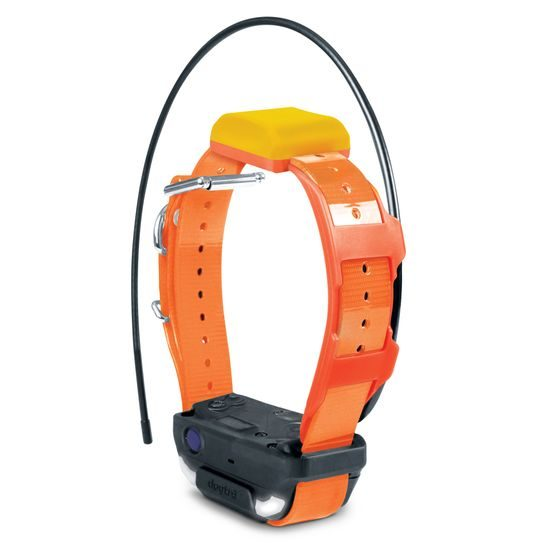
\includegraphics[width=\linewidth]{dogtra.jpg}
        \caption{Odbiornik}
        \label{fig:dogtra-receiver}
    \end{subfigure}
    \hfill
    \begin{subfigure}{0.48\linewidth}
        \centering
        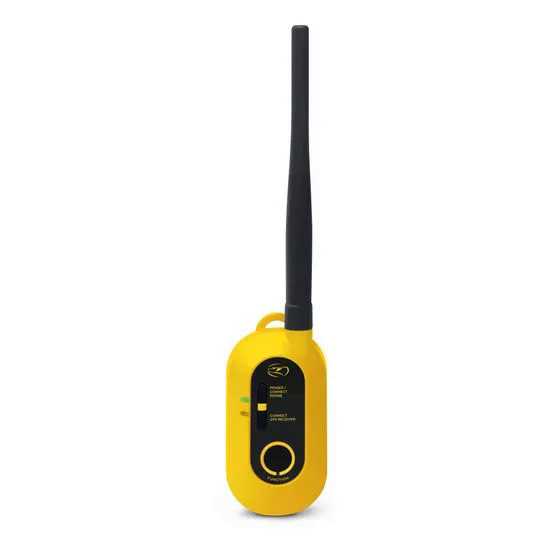
\includegraphics[width=\linewidth]{dogtraremote.png}
        \caption{Pilot zdalnego sterowania}
        \label{fig:dogtra-remote}
    \end{subfigure}
    \caption{Dogtra Pathfinder 2}
    \label{fig:dogtra}
\end{figure}

\subsection*{Dogtrace DOG GPS X25}

Jedynie nieznacznie różnym podejściem wykazała się firma Dogtrace, która w swoim rozwiązaniu
zdecydowała się zrezygnować z konieczności użycia smartfona. X25 składa się z identycznego
funkcjonalnie nadajnika oraz znacznie rozbudowanego odbiornika - wielkości mniejszego smartfona -
który na wbudowanym wyświetlaczu LCD pokazuje kierunek i odległość do nadajnika (rysunek~\ref{fig:dogtrace-x25}). Czeska firma
udostępniła lepszej jakości informacje o funkcjonowaniu swojego produktu. Z oferty na stronie
internetowej\footnote{\url{https://www.obroza-elektryczna.pl/dogtrace-dog-gps-x25}} dowiadujemy
się, że:
\begin{itemize}
    \item możliwe jest śledzenie do 19 psów jednocześnie,
    \item bateria nadajnika i odbiornika powinna wystarczyć na ponad 40 godzin pracy (Li-Pol
          1900~mAh),
    \item pozycjonowanie modułów zapewnia skorzystanie z kilku systemów: GPS, GALILEO, GLONASS,
          a nadajnik z odbiornikiem łączą się po LoRa,
    \item deklarowany zasięg to 20~km dla komunikacji ,,w linii wzroku'',
    \item pełna zanurzalność nadajnika i odbiornika.
\end{itemize}

Dodatkowo dostępne są funkcje takie jak: KOMPAS (kierunek na północ magnetyczną), BEEPER
(wykrywanie ruchu lub bezruchu psa), FENCE (okrągły płot - akustyczna granica wyznaczająca
przestrzeń dla psa), WAYPOINT (możliwość zapisania 4 współrzędnych GPS odbiornika i nawigacja
do tych punktów), tryb CAR (umożliwiający korzystanie z odbiornika w pojeździe) oraz sygnał
dźwiękowy zastępujący gwizdek (3 różne dźwięki do wyboru).

% TODO: Skopiuj plik Dogtrace.png do katalogu img/
\begin{figure}[!h]
    \label{fig:dogtrace-x25}
    \centering
    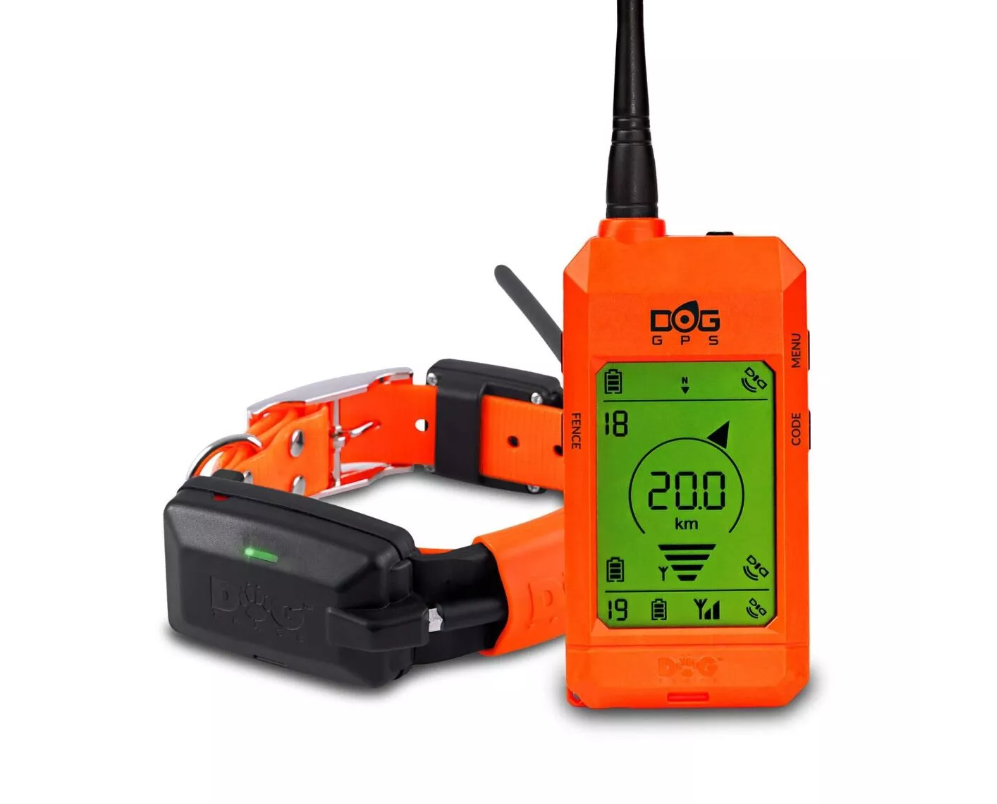
\includegraphics[width=0.5\linewidth]{Dogtrace.png}
    \caption{Dogtrace DOG GPS X25}
\end{figure}

\subsection*{Porównanie z proponowanym rozwiązaniem}

Oba opisane systemy reprezentują podejście typowe dla komercyjnych rozwiązań myśliwskich:
dedykowany sprzęt, bezpośrednia komunikacja nadajnik-odbiornik oraz wysoka cena zakupu.
Proponowany w niniejszej pracy system różni się od nich pod trzema istotnymi względami.

Po pierwsze, komunikacja opiera się na sieci typu mesh, w której każdy węzeł może pełnić
rolę przekaźnika. Oznacza to, że zasięg systemu nie jest ograniczony odległością między
nadajnikiem a odbiornikiem, lecz może być rozszerzany przez dodawanie kolejnych węzłów
pośredniczących - co nie jest możliwe w architekturze punkt-punkt stosowanej przez Dogtrę
i Dogtrace.

Po drugie, system zbudowany jest z ogólnodostępnych komponentów elektronicznych, co 
przekłada się na znacząco niższy koszt w porównaniu z dedykowanym sprzętem komercyjnym.

Po trzecie, liczba węzłów sieci jest nieograniczona przez architekturę systemu, podczas gdy
rozwiązania komercyjne narzucają sztywny limit (21 węzłów dla Dogtra, 19 dla Dogtrace).

Zestawienie kluczowych cech wszystkich trzech rozwiązań przedstawia tabela~\ref{tab:porownanie}.

\begin{table}[!h]
    \caption{Porównanie systemów śledzenia psów myśliwskich}
    \label{tab:porownanie}
    \centering
    \begin{tabular}{|l|c|c|c|}
        \hline
        \textbf{Cecha} & \textbf{Dogtra Pathfinder 2} & \textbf{Dogtrace X25} & \textbf{Proponowany system} \\
        \hline
        Architektura sieci      & punkt-punkt & punkt-punkt & mesh \\
        Zasięg                  & $\sim$14~km & $\sim$20~km & $\geq$2~km\footnotemark[1] \\
        Maks. liczba węzłów     & 21          & 19          & nieograniczona\footnotemark[2] \\
        Aktualizacja pozycji    & co 2~s      & co 3~s      & $\leq$3~s \\
        Geofencing              & tak         & tak         & tak \\
        Kształt strefy          & dowolny wielokąt & okrąg  & dowolny wielokąt \\
        Ochrona                 & IPX9K       & IP68        & IP65 \\
        Koszt                   & 2500 PLN    & 2300 PLN    & 400 PLN\footnotemark[3] \\
        \hline
    \end{tabular}
\end{table}
\footnotetext[1]{Topologia mesh pozwala na rozszerzanie zasięgu przez rozmieszczenie dodatkowych węzłów pośredniczących - podana wartość dotyczy komunikacji między sąsiednimi węzłami sieci.}
\footnotetext[2]{Nieograniczona z punktu widzenia architektury systemu - w praktyce ogranicza ją przepustowość współdzielonego kanału radiowego: wraz ze wzrostem liczby węzłów rośnie ruch w sieci, co może prowadzić do wzrostu zajętości kanału (ograniczonej prawnie).}
\footnotetext[3]{+ 200~PLN za każdy kolejny węzeł.}

\newpage
\section{Projekt}

Niniejszy rozdział opisuje decyzje projektowe podjęte w trakcie realizacji systemu,
obejmując wybór technologii komunikacji radiowej i platformy sprzętowej, konfigurację
sieci mesh oraz architekturę aplikacji mobilnej.

\subsection*{Wybór technologii}

Dobór platformy sprzętowej poprzedzono wyborem techniki modulacji. W projekcie wykorzystano technologię
LoRa. Poniżej przedstawiono krótki opis teoretyczny oraz uzasadnienie wyboru.

\subsection*{Modulacja LoRa i technika Chirp Spread Spectrum}

LoRa (ang.\ \textit{Long Range}) to technika modulacji radiowej, która pozwala na przesyłanie
niewielkich pakietów danych na bardzo duże odległości - nawet kilkanaście kilometrów - przy
minimalnym zużyciu energii.\footnote{\url{https://www.gov.pl/web/instytut-lacznosci/lora-pod-lupa}}
Jej zamysł opiera się na technice modulacji CSS (ang.\ \textit{Chirp Spread Spectrum}) lub FSCM
(ang.\ \textit{Frequency Shift Chirp Modulation})~\cite{vangelista2017lora}. Polega ona na
kodowaniu sygnału przez cykliczne przesunięcie punktu startowego chirpa. Wspomniany chirp to
,,blok'' sygnału o liniowo zmiennej częstotliwości.

Modulację LoRa opisują trzy główne parametry:
\begin{itemize}
    \item \textbf{Współczynnik rozpraszania SF} (ang.\ \textit{Spreading Factor}) - określa
          liczbę chirpów przypadających na jeden symbol. Im wyższy SF, tym dłuższy czas transmisji
          symbolu, ale też lepsza czułość odbiornika i większy zasięg. W praktyce stosuje się
          wartości od 7 do 12.

    \item \textbf{Szerokość pasma BW} (ang.\ \textit{Bandwidth}) - określa zakres częstotliwości
          zajmowany przez sygnał. Szersza szerokość pasma oznacza krótszy czas transmisji symbolu
          przy tym samym SF, ale też wyższy poziom szumów i mniejszy zasięg. W praktyce do wyboru
          są częstotliwości 125, 250 lub 500~kHz.

    \item \textbf{Współczynnik kodowania CR} (ang.\ \textit{Coding Rate}) - określa nadmiarowość
          kodu korekcji błędów. Wyższy CR zwiększa odporność na błędy transmisji kosztem wydajności.
\end{itemize}

Przepustowość bitową modulacji LoRa wyraża wzór:\footnote{\url{https://josefmtd.com/2018/08/14/spreading-factor-bandwidth-coding-rate-and-bit-rate-in-lora-english/}}

\begin{equation}
    R_b = SF \cdot \frac{BW}{2^{SF}} \cdot \frac{CR}{4+CR}
    \label{eq:lora-bitrate}
\end{equation}

Kluczową zaletą CSS jest odporność na zakłócenia wąskopasmowe poprzez rozłożenie energii sygnału
na całe dostępne pasmo. Efekt Dopplera (istotny przy komunikacji w ruchu) również jest ograniczony.
Wynika to z tego, że odczyt symbolu polega w skrócie na mnożeniu odebranego sygnału przez chirp
bazowy i wykonaniu FFT (ang.\ \textit{Fast Fourier Transform}). Powstały w wyniku pik widmowy jest
jedynie przesunięty i przy prędkościach spotykanych w praktyce nie spowoduje błędu dekodowania.

\subsection*{Wybór platformy sprzętowej}

W projekcie rozważono możliwość wykorzystania różnych platform sprzętowych z modułami radiowymi LoRa:
\begin{enumerate}
    \item \textbf{Raspberry Pi z modułami LoRa} - mimo licznych zalet, takich jak bogate wsparcie,
          względnie wysoka moc obliczeniowa oraz elastyczność, przeważyły wady, które wykluczyły to
          rozwiązanie: zbyt duże zużycie energii, duże rozmiary, brak wodoszczelności. Podobne
          argumenty zdecydowały o wyeliminowaniu platformy \textit{Arduino~Uno/Nano z modułem LoRa}.
    \item \textbf{ESP32 z modułami LoRa} - w szczególności rozważono \textit{Heltec ESP32 LoRa},
          czyli płytkę z wbudowanym modułem LoRa i wyświetlaczem OLED. Produkt ten posiada wiele
          cech wypełniających wymagania projektu (wbudowany moduł Bluetooth i LoRa, niskie zużycie
          energii, niski koszt), jednak o odrzuceniu tej platformy zadecydowały pragmatyczne względy: 
          brak wodoszczelności - ewentualna konieczność druku 3D obudowy, a osiądnięcie IP65 w drukowanej 
          obudowie wymaga m.in. dedykowanych złączy kablowych, co znacznąco podnosi poziom skomplikowania projektu.
    \item \textbf{Meshtastic na dedykowanym sprzęcie LoRa} - otwartoźródłowa platforma łącząca
          firmware dla modułów radiowych LoRa z ekosystemem aplikacji klienckich. Tworzy
          zdecentralizowaną sieć mesh w paśmie ISM bez infrastruktury zewnętrznej, każdy węzeł
          automatycznie retransmituje pakiety pozostałych, rozszerzając zasięg sieci wraz
          z liczbą urządzeń. Platforma udostępnia publiczne API w postaci aplikacji Android
          \texttt{com.geeksville.mesh}\footnote{Repozytorium aplikacji Meshtastic na Android:
          \url{https://github.com/meshtastic/Meshtastic-Android}. Dokumentacja API:
          \url{https://meshtastic.org/docs/development/firmware/build/}.} oraz eksportuje 
          interfejs AIDL\footnote{AIDL (ang.\ \textit{Android Interface Definition Language}) to mechanizm
          systemu Android umożliwiający komunikację między procesami.} umożliwiający aplikacjom
          trzecim odczyt danych telemetrycznych - w tym pozycji GPS węzłów.
          Sprzęt kompatybilny z Meshtastic jest ogólnodostępny i tani, a samo oprogramowanie
          bezpłatne. Spośród rozważanych opcji platforma ta najlepiej spełnia wymagania projektu.
\end{enumerate}

Wybór platformy Meshtastic podyktowany był przede wszystkim dostępnością dedykowanego sprzętu
spełniającego wymagania wodoszczelności oraz możliwością integracji z aplikacją mobilną przez
publiczne API. W ramach platformy wybór padł na:
\begin{itemize}
    \item \textit{T-Beam} - popularna platforma oparta na ESP32 z wbudowanym modułem GPS, anteną
          LoRa oraz akumulatorem. Posiada duży akumulator oraz otwarte piny, które zostawiają
          szerokie pole manewru do rozwoju tego węzła w roli stacji bazowej.
    \item \textit{T-2000-E} - kompaktowe urządzenie oferujące wodoszczelność (IP65), wbudowany GPS
          oraz zoptymalizowaną żywotność baterii. Wymiary i kształt są spełniają wymagania projektu, bo
          urządzenie ma wymiary dwóch złożonych kart bankowych - 6,5x85x55mm i waży 32 g.
\end{itemize}

Obie platformy przedstawia rysunek~\ref{fig:platformy}.

\begin{figure}[H]
    \centering
    \begin{subfigure}{0.48\linewidth}
        \centering
        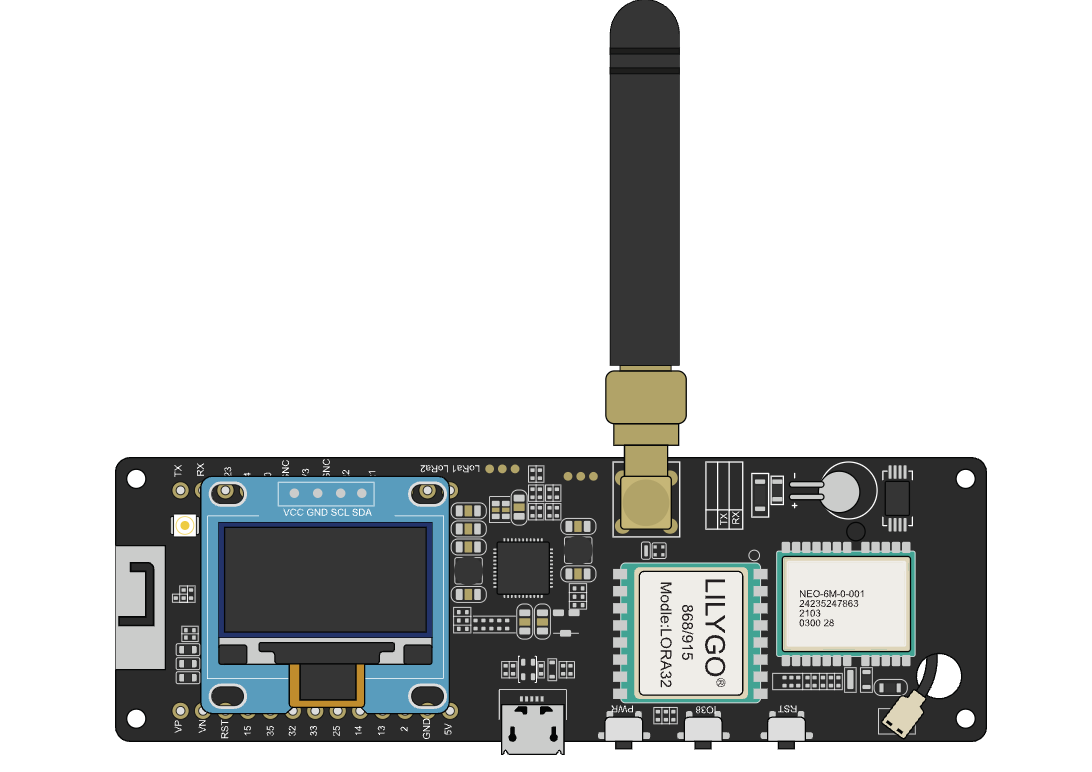
\includegraphics[width=\linewidth]{tbeam.png}
        \caption{T-Beam - węzeł stacji bazowej}
        \label{fig:tbeam}
    \end{subfigure}
    \hfill
    \begin{subfigure}{0.48\linewidth}
        \centering
        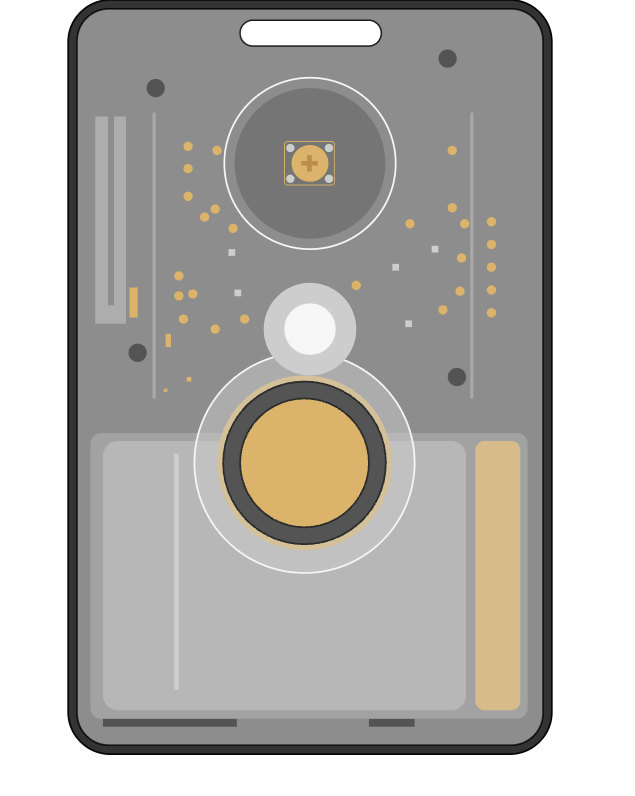
\includegraphics[width=\linewidth]{tracker-t1000-e.png}
        \caption{T1000-E - węzeł obroży}
        \label{fig:t1000e}
    \end{subfigure}
    \caption{Wybrane platformy sprzętowe Meshtastic}
    \label{fig:platformy}
\end{figure}

Otwartoźródłowy charakter projektu stwarza możliwość implementacji rozszerzeń dla węzłów sieci
w postaci modułów. Dzięki temu wybór Meshtastic jako platformy sprzętowej nie ograniczy projektu
do domyślnie dostępnych funkcji. Spośród dostępnych konfiguracji radiowych można wybrać parametry
dla modulacji LoRa. Zostały one zestawione w tabeli~\ref{tab:lora-presets}.\footnote{\url{https://meshtastic.org/docs/software/site-planner/}}

\begin{table}[!h]
    \caption{Predefiniowane ustawienia kanałów LoRa w Meshtastic}
    \label{tab:lora-presets}
    \centering
    \begin{tabular}{|l|c|c|c|}
        \hline
        \textbf{Ustawienie} & \textbf{BW [kHz]} & \textbf{SF} & \textbf{CR} \\
        \hline
        ShortTurbo   & 500 & 7  & 4/5 \\
        ShortFast    & 250 & 7  & 4/5 \\
        ShortSlow    & 250 & 8  & 4/5 \\
        MediumFast   & 250 & 9  & 4/5 \\
        MediumSlow   & 250 & 10 & 4/5 \\
        LongFast     & 125 & 11 & 4/5 \\
        LongModerate & 125 & 11 & 4/8 \\
        LongSlow     & 125 & 12 & 4/8 \\
        \hline
    \end{tabular}
\end{table}


Zazwyczaj do konfiguracji sieci Meshtastic używa się następujących parametrów: $SF=12$,
$BW=125$~kHz oraz $CR=4/8$. Podstawiając je do wzoru~(\ref{eq:lora-bitrate}) otrzymuje się przepustowość
na poziomie 250~bps. Jest ona w zupełności wystarczająca do przesyłania krótkich pakietów
zawierających współrzędne GPS.

\subsection*{Konfiguracja sieci Meshtastic}

Sieć Meshtastic skonfigurowano tak, aby wszystkie węzły mogły przesyłać między sobą informacje
o swoim położeniu GPS. W sieci Meshtastic informacje o pozycji GPS są przesyłane jako część telemetrii węzła. Telemetria
jest automatycznie udostępniana wszystkim węzłom w sieci, które używają tego samego kanału PRIMARY
(lub kanału wtórnego z włączoną pozycją), mają zgodne ustawienia LoRa (częstotliwość, modem preset)
oraz są w zasięgu (bezpośrednio lub przez pośrednie węzły). Schemat sieci przedstawia rysunek~\ref{fig:schematSieci}.

\begin{figure}[H]
    \label{fig:schematSieci}
    \centering
    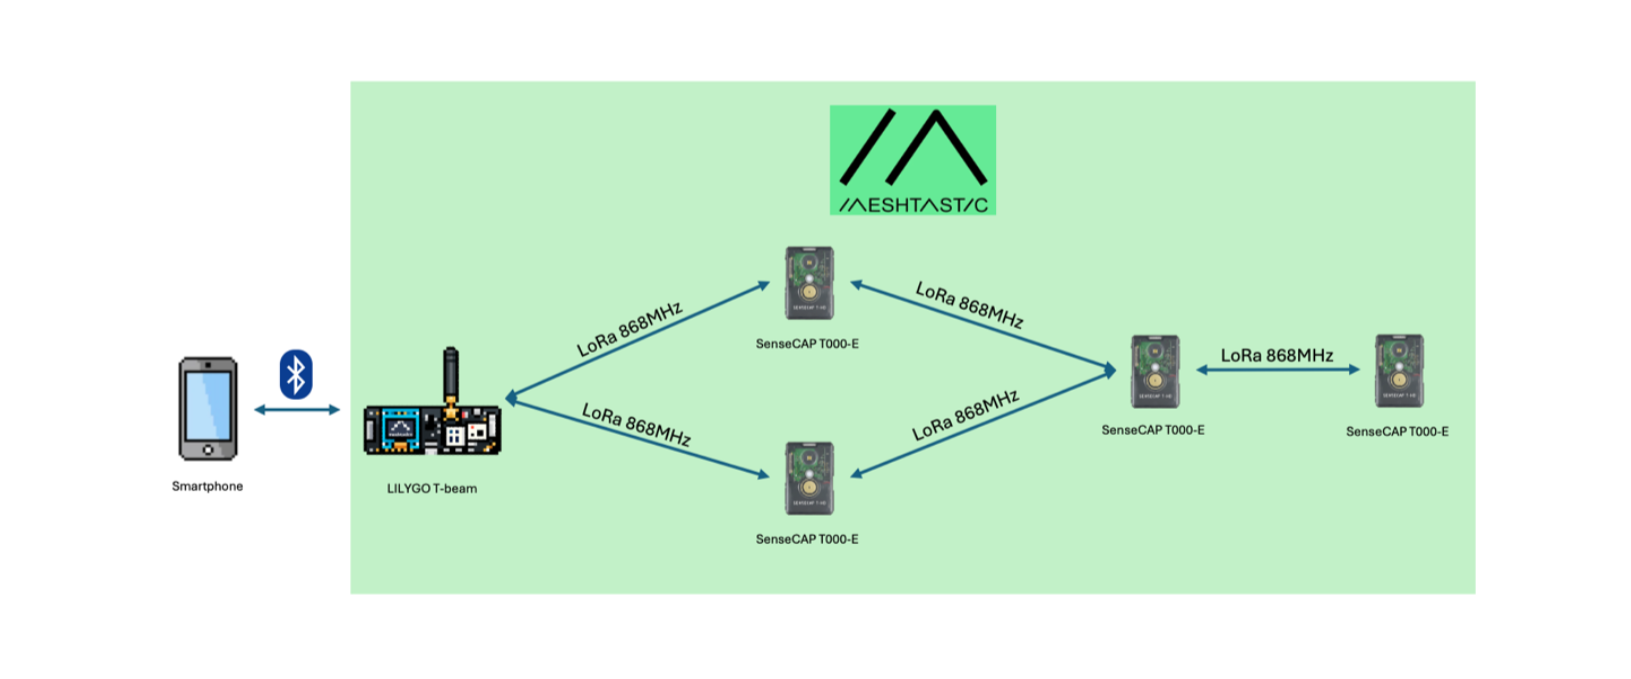
\includegraphics[width=0.9\linewidth]{schematSieci.png}
    \caption{Schemat sieci Meshtastic z pięcioma węzłami}
\end{figure}

\paragraph{Konfiguracja - prywatne kanały.}

Aby udostępniać pozycję wyłącznie węzłom należącym do sieci prywatnej, konieczne było zastosowanie
prywatnego kanału. Konfiguracja przebiegła następująco:

\begin{enumerate}
    \item \textbf{Wyłączono pozycję na kanale PRIMARY}:
          Settings $\rightarrow$ Radio Config $\rightarrow$ Channels $\rightarrow$ Channel 0 (PRIMARY)
          $\rightarrow$ Position Sharing: \textbf{WYŁĄCZONE}.

    \item \textbf{Utworzono prywatny kanał}:
          Settings $\rightarrow$ Radio Config $\rightarrow$ Channels $\rightarrow$ \textbf{Add Channel},
          z następującymi parametrami:
          \begin{itemize}
              \item \textbf{Channel Name}: \texttt{Reja}
              \item \textbf{PSK}: wspólny klucz szyfrowania
              \item \textbf{Position Sharing}: \textbf{WŁĄCZONE}
              \item \textbf{Position Precision}: najwyższy poziom precyzji 32-bity
                    (deklaruje dokładność co do metra)
          \end{itemize}

    \item \textbf{Dodano ten sam kanał do wszystkich węzłów w grupie}: wszystkie węzły mają
          identyczną nazwę kanału \texttt{Reja} oraz identyczny klucz PSK.
\end{enumerate}



\section{Aplikacja mobilna MeshTracker}

\subsection*{Architektura}

Aplikacja wykorzystuje architekturę opartą na wzorcu \textbf{MVVM
(Model-View-ViewModel)}\footnote{\url{https://learn.microsoft.com/pl-pl/dotnet/architecture/maui/mvvm}}
z osobnymi, dodatkowymi warstwami odpowiedzialnymi za komunikację zewnętrzną z aplikacją Meshtastic.
Jest to standardowo wykorzystywany wzorzec, który oddziela logikę działania aplikacji od interfejsu
użytkownika. Warstwa \textit{View} odpowiada za renderowanie interfejsu i reagowanie na zdarzenia
użytkownika, warstwa \textit{ViewModel} przechowuje stan ekranu i przetwarza dane z modelu,
natomiast warstwa \textit{Model} reprezentuje dane domenowe - węzły, strefy geofencingu
i zdarzenia przekroczenia granic. Komunikacja z siecią Meshtastic odbywa się przez dedykowaną
warstwę serwisową, która izoluje resztę aplikacji od szczegółów protokołu AIDL (rysunek~\ref{fig:architektura}).

\begin{figure}[H]
    \label{fig:architektura}
    \centering
    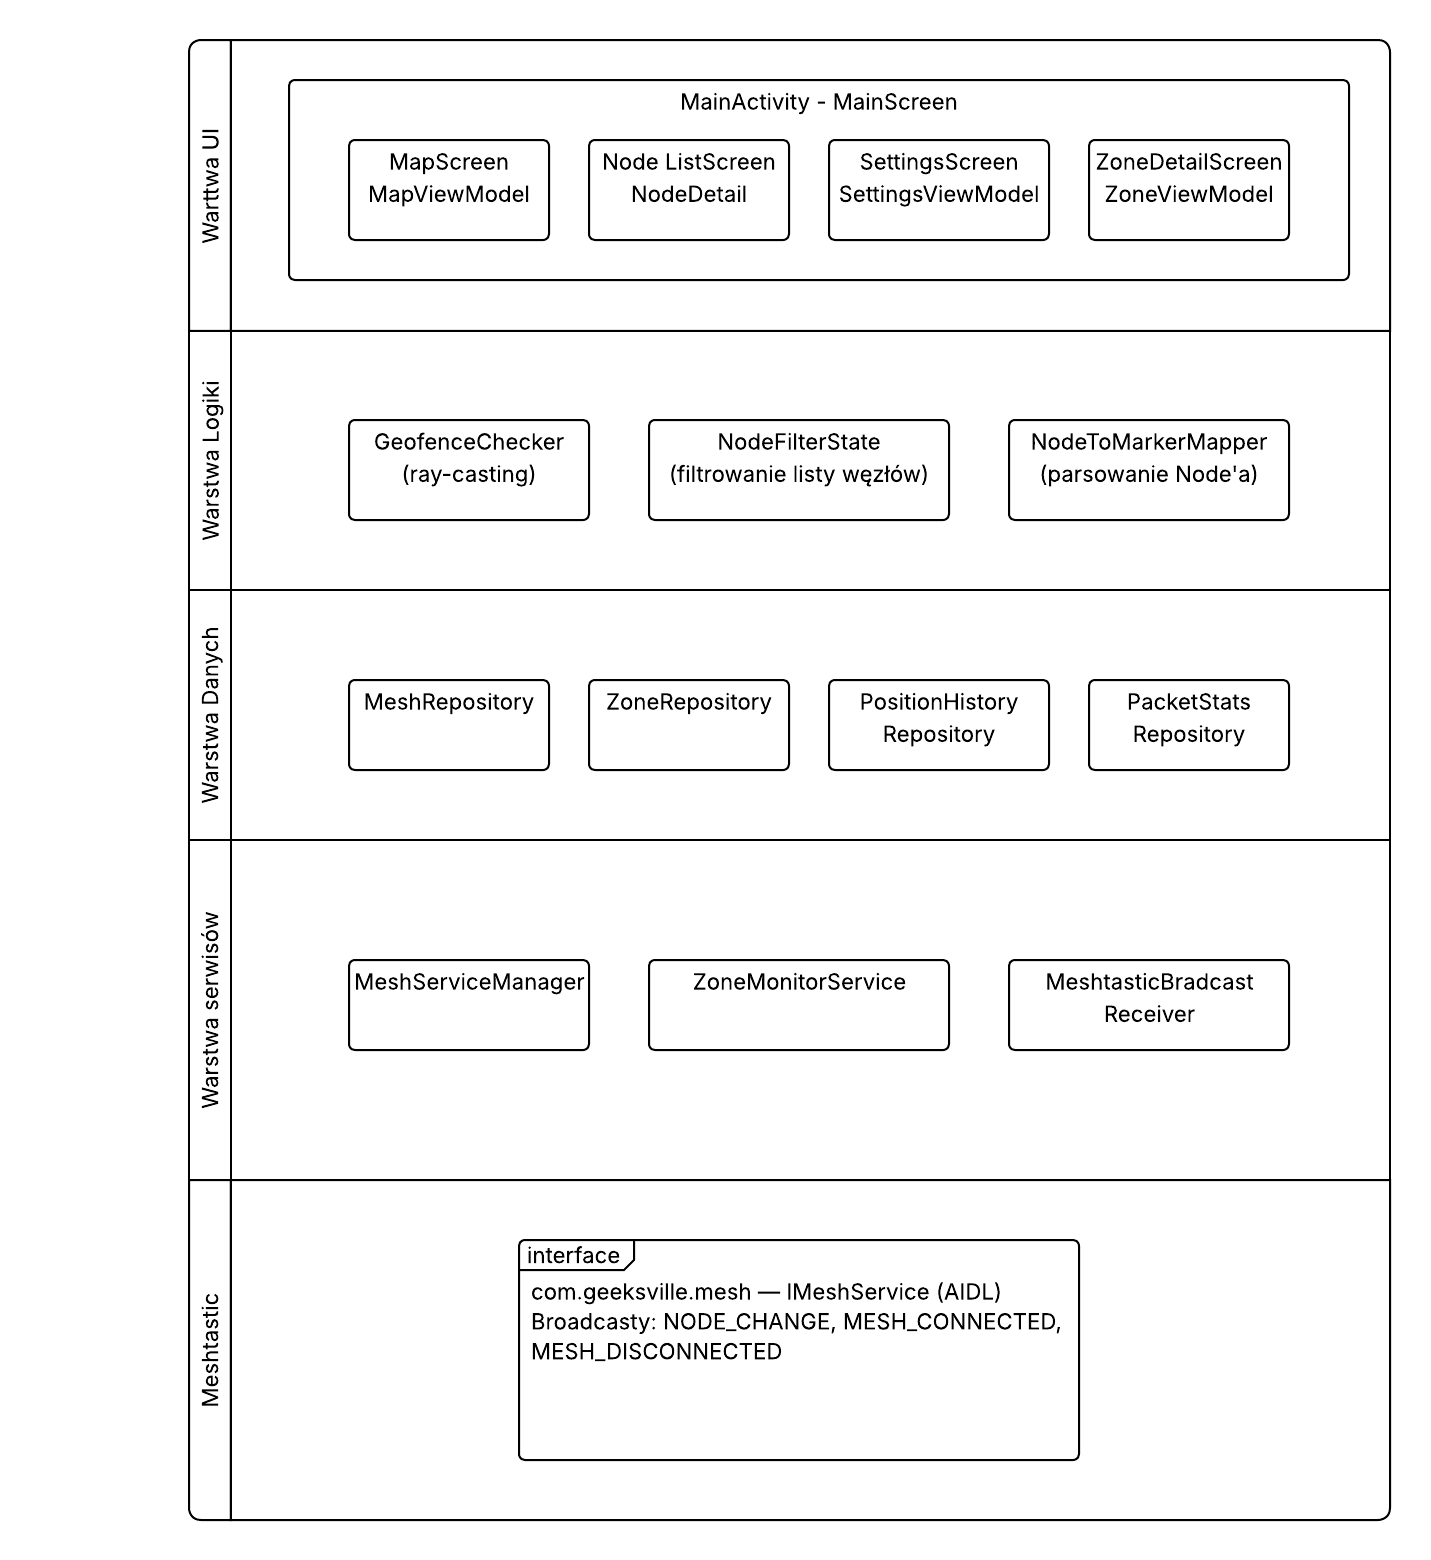
\includegraphics[width=0.8\linewidth]{ArchitectureWhiteBackground.png}
    \caption{Architektura aplikacji MeshTracker}
\end{figure}

\subsection*{Przegląd ekranów aplikacji}

Interfejs użytkownika aplikacji MeshTracker zorganizowany jest wokół trzech głównych ekranów. Wszystkie
dostępne są przez pasek nawigacyjny w dolnej części ekranu: \textbf{mapy}, \textbf{listy węzłów} oraz
\textbf{ustawień}. 

Każdy ekran posiada dedykowany ViewModel odpowiedzialny
za logikę prezentacji, zgodnie z przyjętym wzorcem MVVM. Komponenty współdzielone między
ekranami, takie jak pasek stanu połączenia, wydzielono do osobnego pakietu \texttt{components}.
Wygląd aplikacji definiowany jest przez pakiet \texttt{theme}, zawierający paletę kolorów,
typografię oraz motyw Material Design 3. Strukturę pakietu \texttt{ui} ilustruje rysunek~\ref{fig:ui-structure}.

\begin{figure}[H]
    \centering
    \scriptsize
    \dirtree{%
        .1 ui/.
        .2 MainScreen.kt.
        .2 components/.
        .3 ConnectionStatusBar.kt.
        .2 map/.
        .3 MapScreen.kt.
        .3 MapViewModel.kt.
        .2 nodes/.
        .3 NodeDetailScreen.kt.
        .3 NodeFilterState.kt.
        .3 NodeItem.kt.
        .3 NodeListScreen.kt.
        .2 settings/.
        .3 SettingsScreen.kt.
        .3 SettingsViewModel.kt.
        .2 theme/.
        .3 Color.kt.
        .3 Theme.kt.
        .3 Type.kt.
        .2 zones/.
        .3 ZoneBottomSheet.kt.
        .3 ZoneConfirmDialog.kt.
        .3 ZoneDetailScreen.kt.
        .3 ZoneViewModel.kt.
    }
    \caption{Struktura pakietu \texttt{ui}}
    \label{fig:ui-structure}
\end{figure}

\paragraph{Mapy.}
\texttt{MapScreen} jest głównym ekranem aplikacji. Wyświetla mapę Google Maps,
na której prezentowane są markery węzłów oraz pozycja użytkownika. Każdy marker renderowany
jest jako bitmapa z inicjałami węzła. Kolor markera zależy od roli węzła oraz stanu połączenia.
W prawym górnym rogu markera znajduje się znacznik jakości sygnału. W lewym dolnym rogu ekranu
umieszczono \textit{floating button} otwierający menu geofencingu (rysunek~\ref{fig:map-screen}).

\begin{figure}[!h]
    \centering
    \begin{minipage}{0.48\linewidth}
        \centering
        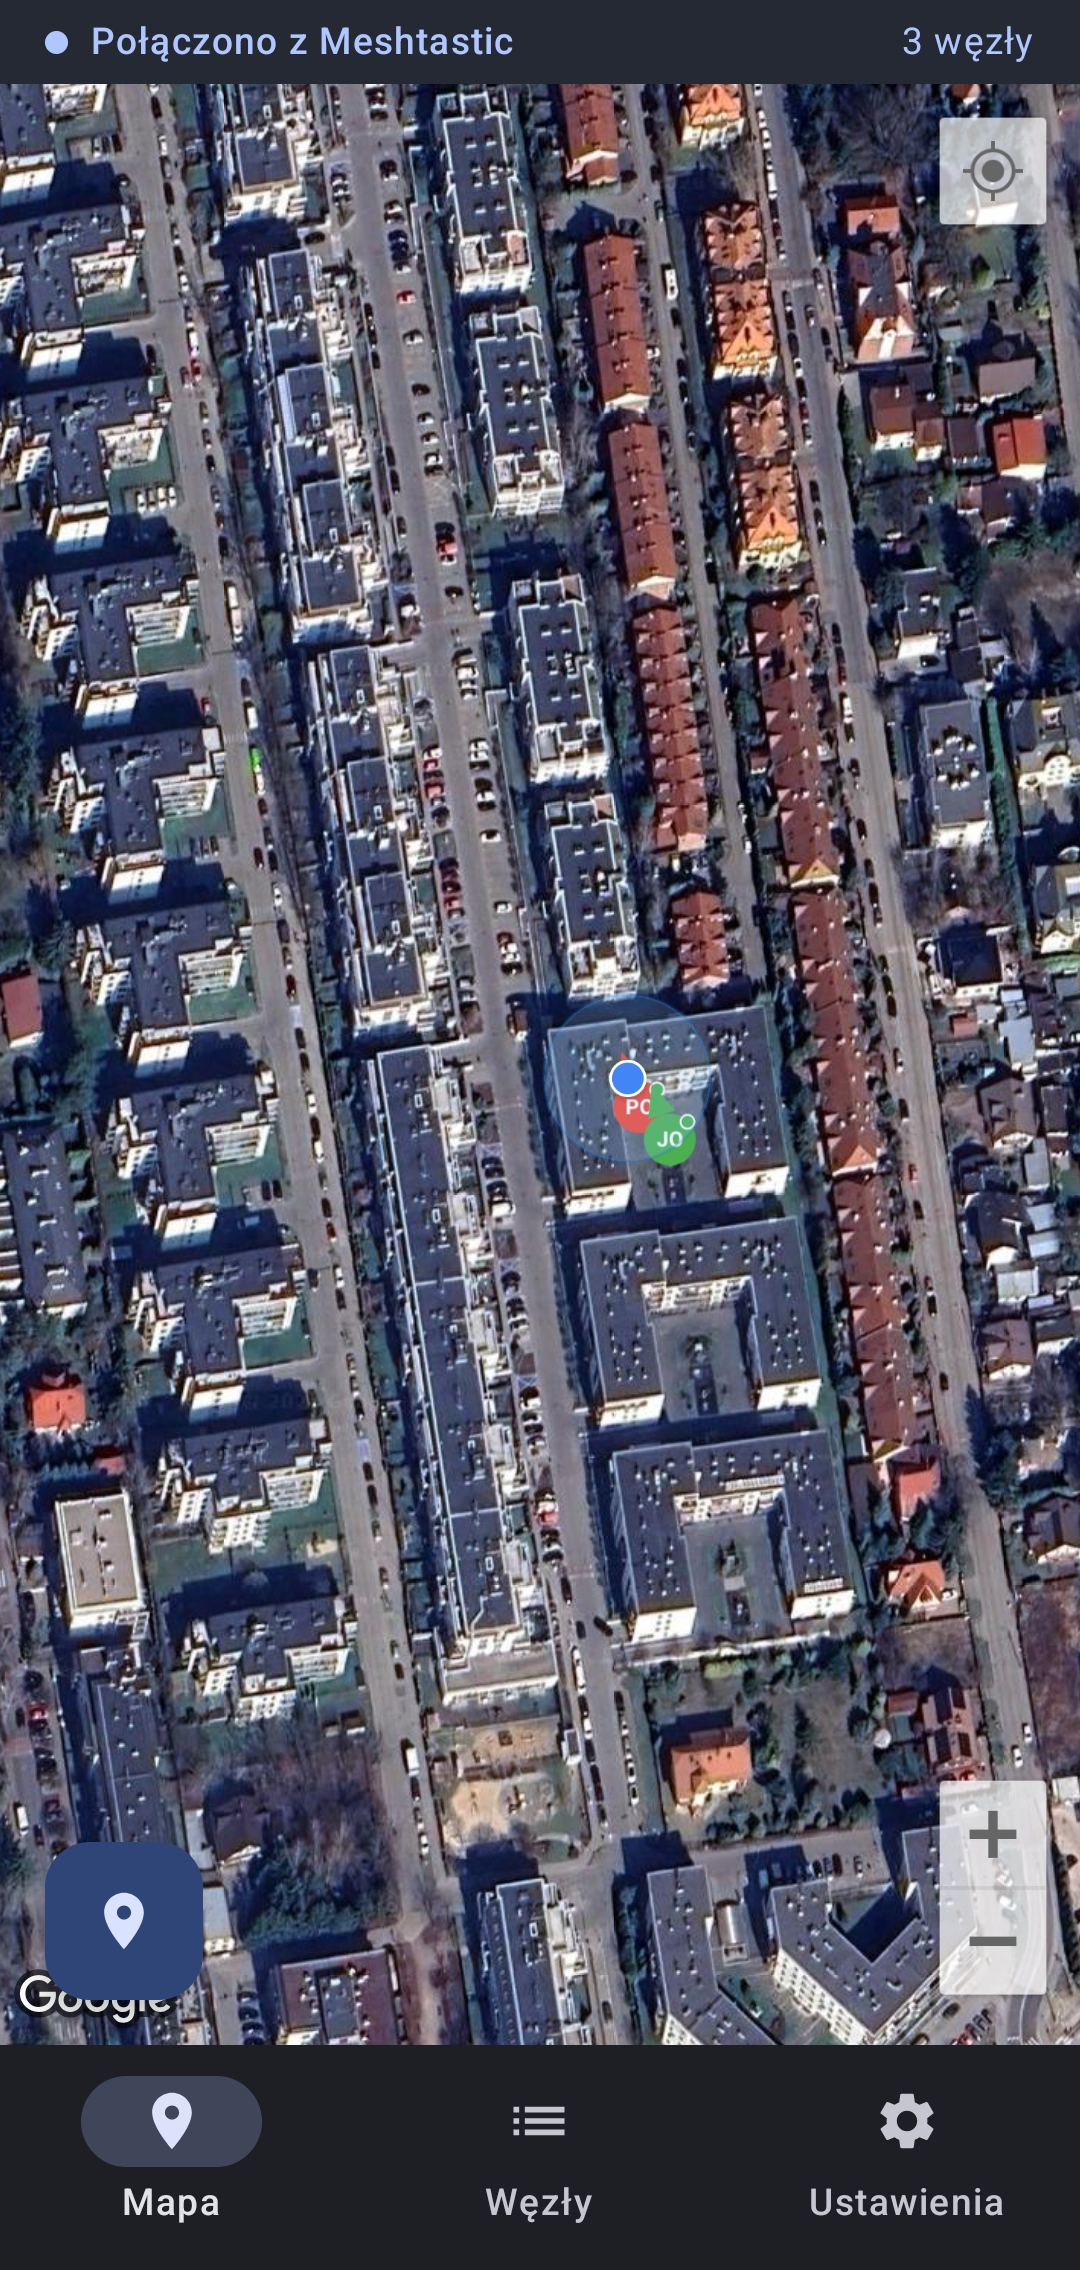
\includegraphics[width=\linewidth]{mapaZblizenie.jpg}
        \captionof{figure}{Ekran mapy aplikacji MeshTracker}
        \label{fig:map-screen}
    \end{minipage}
    \hfill
    \begin{minipage}{0.48\linewidth}
        \centering
        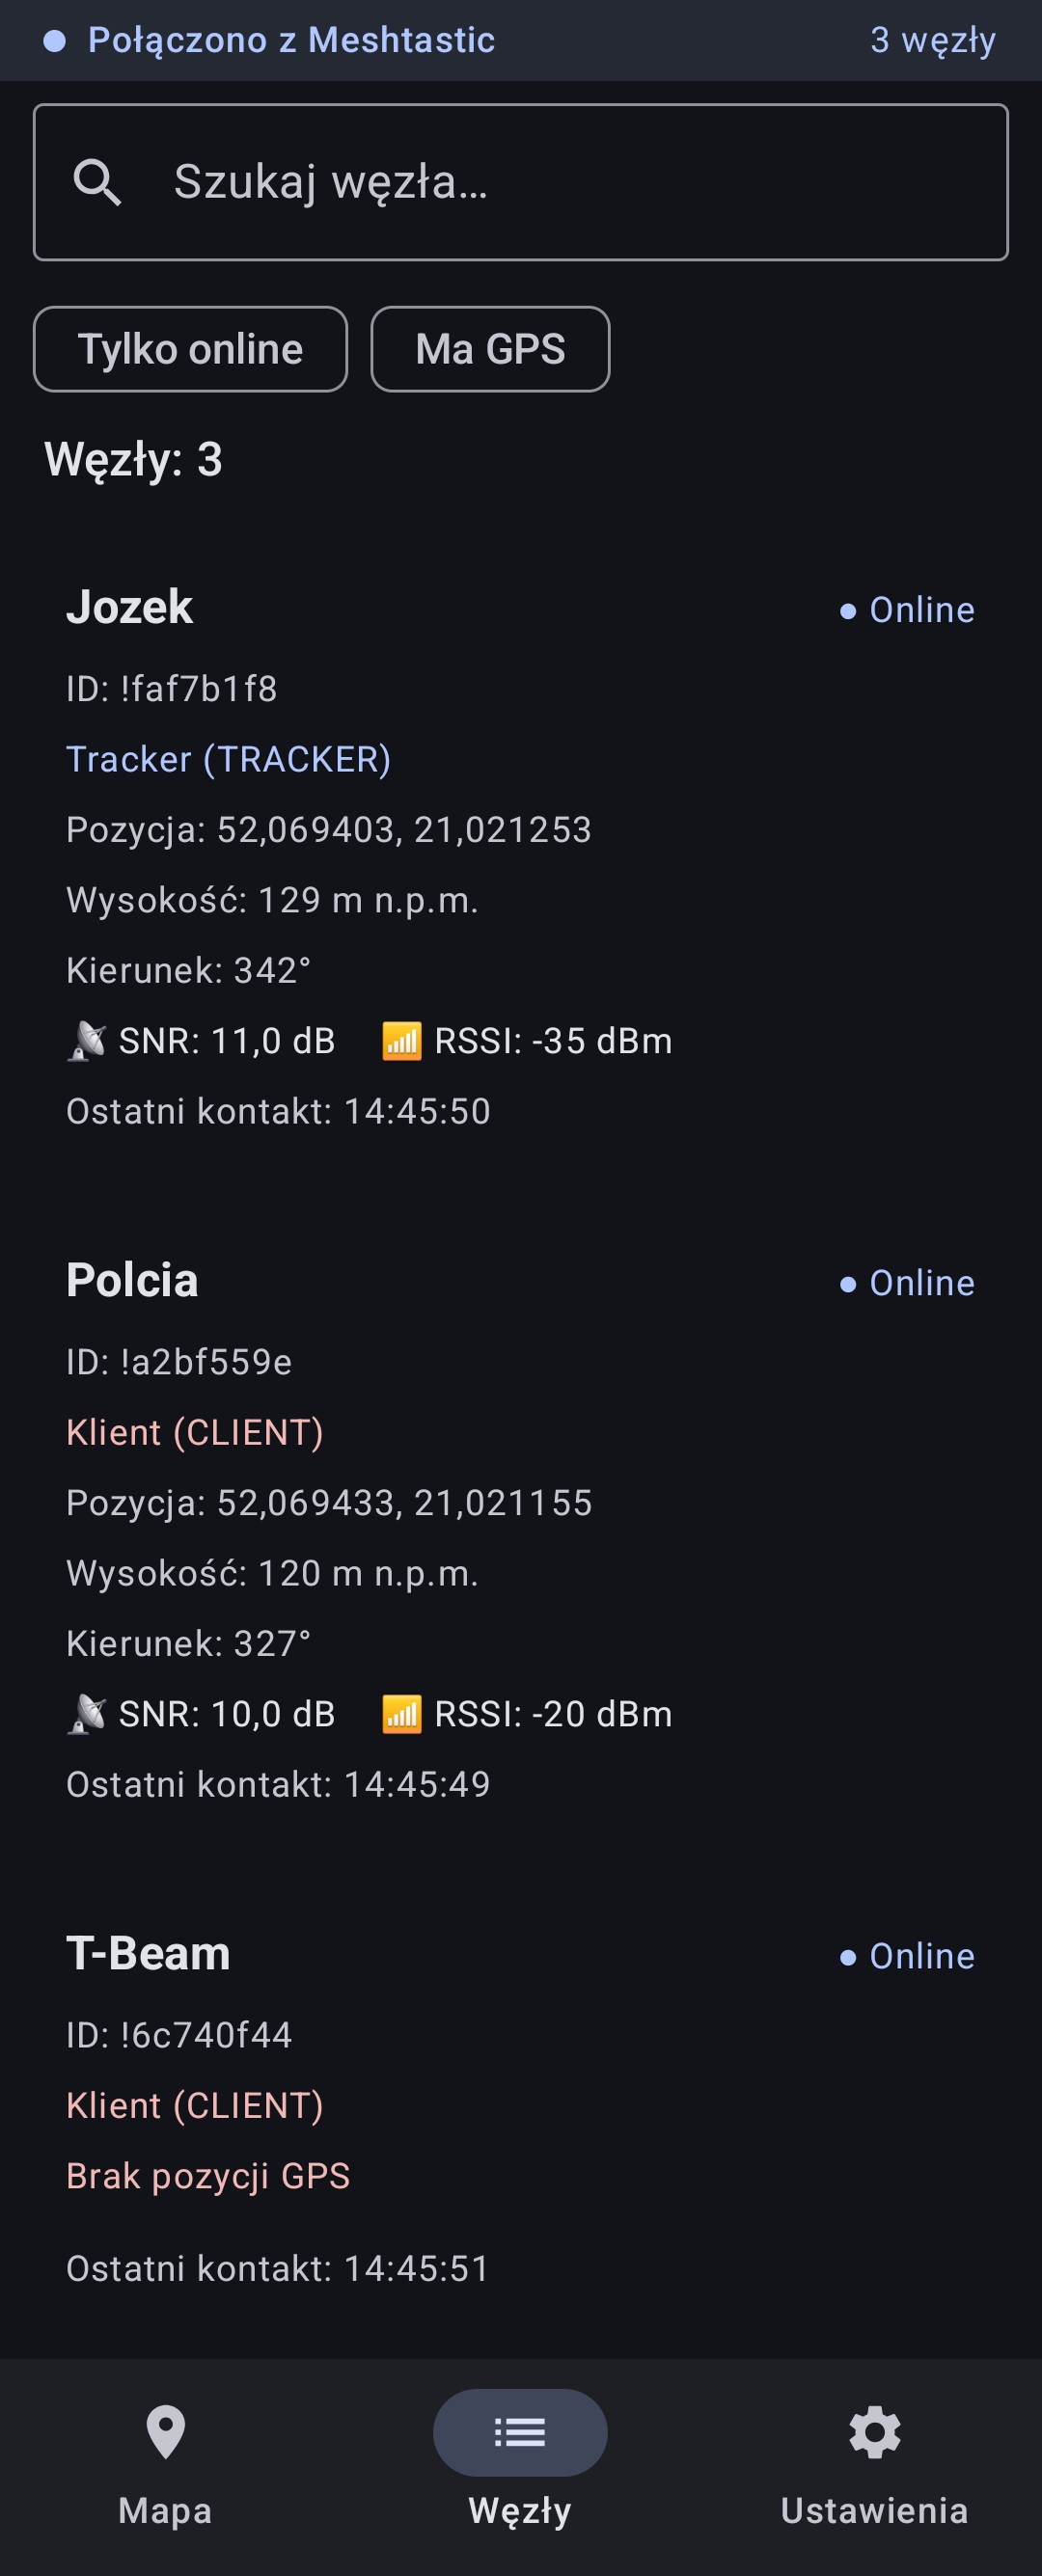
\includegraphics[width=\linewidth]{wezlyLista.jpg}
        \captionof{figure}{Ekran listy węzłów}
        \label{fig:wezly-lista}
    \end{minipage}
\end{figure}


\paragraph{Markery.}

Wizualizacja markerów została zaprojektowana tak, aby w jak najbardziej przejrzysty sposób
prezentować możliwie wiele danych jednocześnie. Kolor markera odpowiada przypisanej mu roli,
a dodatkowa warstwa kolorów reprezentuje stan połączenia węzła z siecią Meshtastic
(rysunek~\ref{fig:markery-kolory}).

\begin{figure}[!h]
    \centering
    \begin{subfigure}{0.48\linewidth}
        \centering
        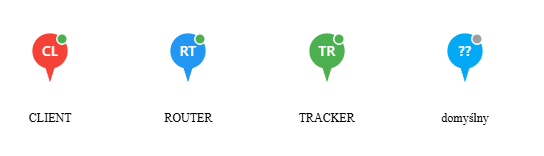
\includegraphics[width=\linewidth]{markeryRole.png}
        \caption{Mapowanie roli węzła do koloru}
        \label{fig:markery-role}
    \end{subfigure}
    \hfill
    \begin{subfigure}{0.48\linewidth}
        \centering
        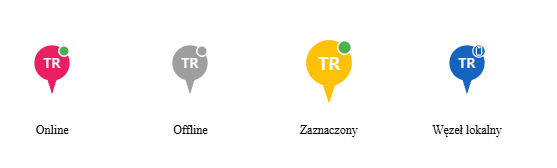
\includegraphics[width=\linewidth]{markeryStanPolaczenia.png}
        \caption{Mapowanie stanu połączenia do koloru}
        \label{fig:markery-stan-polaczenia}
    \end{subfigure}
    \caption{Kodowanie kolorystyczne markerów}
    \label{fig:markery-kolory}
\end{figure}

Węzeł lokalny - czyli ten połączony z telefonem użytkownika bezpośrednio przez Bluetooth -
posiada małą ikonkę telefonu w prawym górnym rogu. Pozostałe węzły mają w tym miejscu kropkę,
której kolor odpowiada jakości połączenia z siecią (zakres SNR\footnote{SNR (ang.\
\textit{Signal-to-Noise Ratio}) - stosunek mocy użytecznego sygnału do mocy szumu,
wyrażony w~dB. Im wyższa wartość, tym lepsze połączenie.} wyrażony w~dB). Strzałka wewnątrz markera wskazuje kierunek
poruszania się węzła (rysunek~\ref{fig:markery-szczegoly}).

\begin{figure}[!h]
    \centering
    \begin{subfigure}{0.48\linewidth}
        \centering
        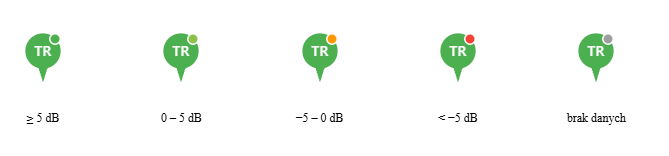
\includegraphics[width=\linewidth]{markeryJakoscPolaczenia.png}
        \caption{Jakość połączenia (SNR) a kolor kropki}
        \label{fig:markery-jakosc-polaczenia}
    \end{subfigure}
    \hfill
    \begin{subfigure}{0.48\linewidth}
        \centering
        
\includegraphics[width=\linewidth]{markeryKierunek.png}
        \caption{Kierunek poruszania się węzła}
        \label{fig:markery-kierunek}
    \end{subfigure}
    \caption{Wizualizacji markerów}
    \label{fig:markery-szczegoly}
\end{figure}

\paragraph{Geofencing.}

Menu stref dostępne jest pod \textit{floating button} w lewym dolnym rogu ekranu mapy.
Strefy składają się z wielokątów, których wierzchołki tworzone są poprzez długie przyciśnięcie
(\textit{long press}) wybranego punktu na mapie. Po dodaniu trzeciego wierzchołka pojawia się
opcja \textbf{Zamknij}, która tworzy strefę z wprowadzonych punktów
(rysunek~\ref{fig:geofencing-tworzenie}).

\begin{figure}[!h]
    \centering
    \begin{subfigure}{0.45\linewidth}
        \centering
        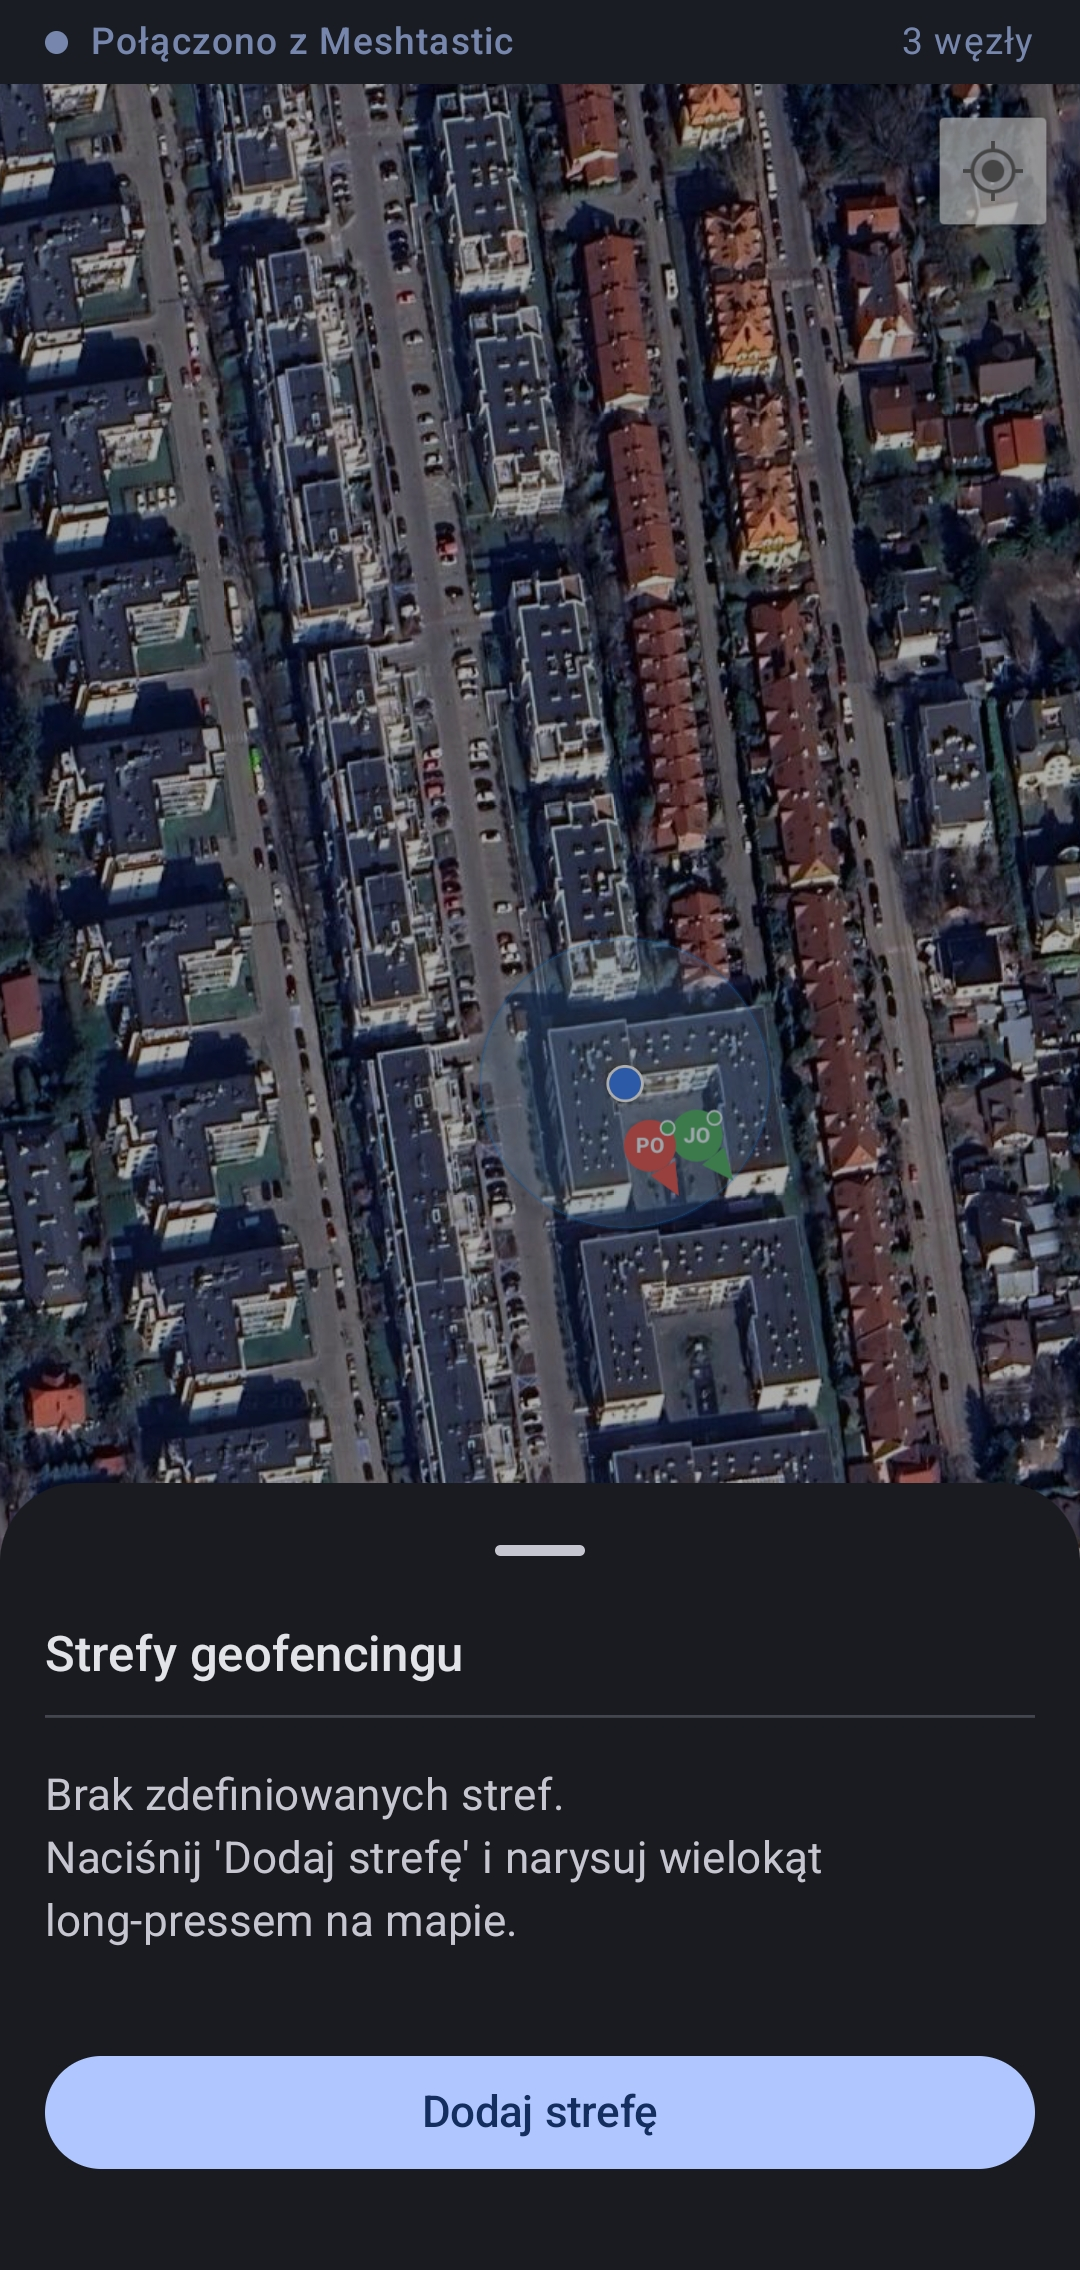
\includegraphics[width=\linewidth]{strefyGeofencing.jpg}
        \caption{Menu geofencingu - widok pusty}
        \label{fig:geofencing-puste}
    \end{subfigure}
    \hfill
    \begin{subfigure}{0.45\linewidth}
        \centering
        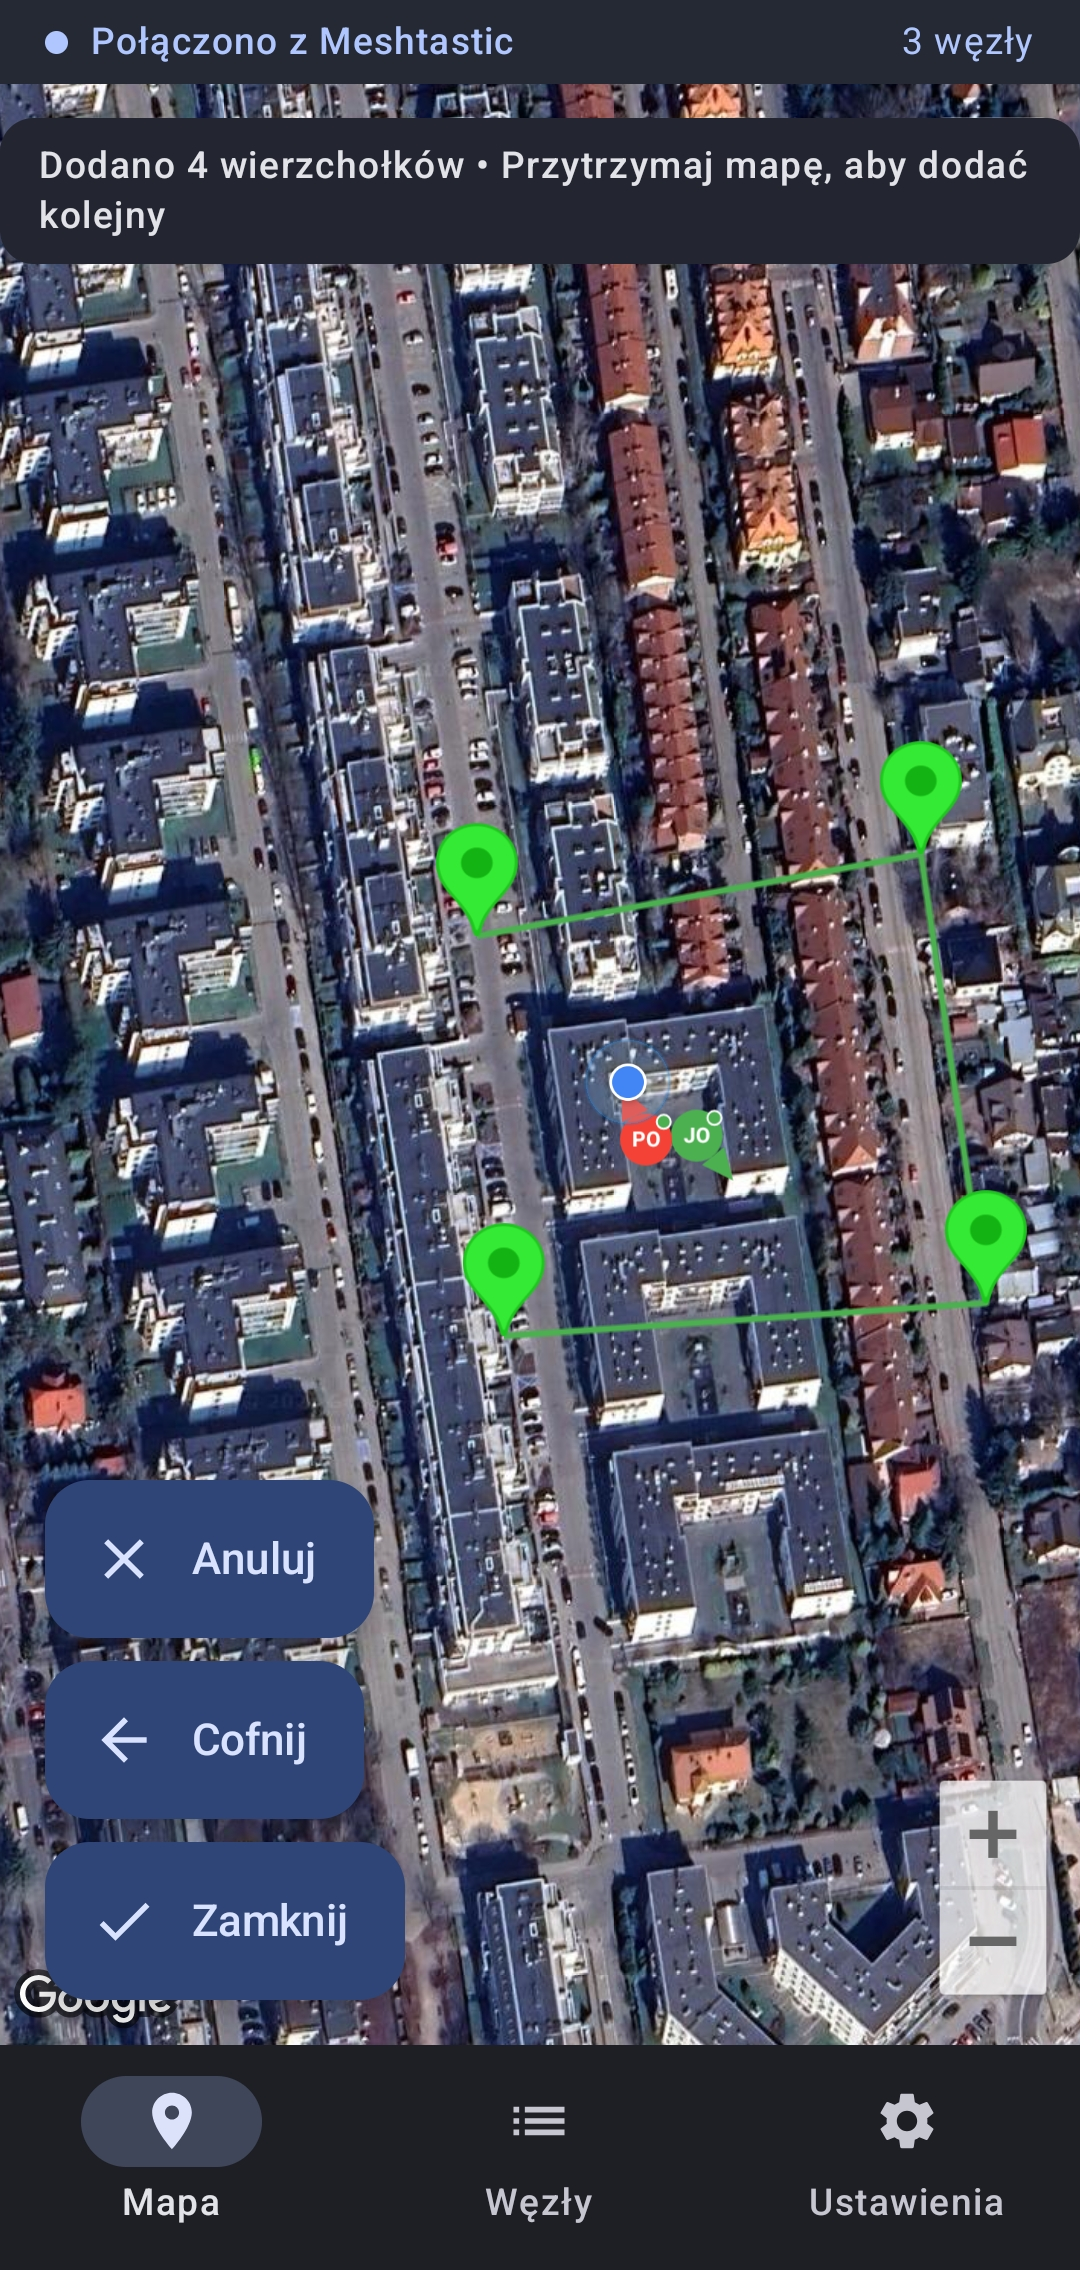
\includegraphics[width=\linewidth]{strefyGeofencingWierzcholki.jpg}
        \caption{Definiowanie wierzchołków strefy}
        \label{fig:geofencing-wierzcholki}
    \end{subfigure}
    \caption{Tworzenie strefy geofencingu}
    \label{fig:geofencing-tworzenie}
\end{figure}

Następnie użytkownik wprowadza nazwę strefy, nadaje jej kolor oraz przypisuje węzły, które
będą wyzwalać zdarzenia wejścia i wyjścia. Dostępne strefy mogą być aktywowane i usuwane
z poziomu listy (rysunek~\ref{fig:geofencing-zarzadzanie}).

\begin{figure}[!h]
    \centering
    \begin{subfigure}{0.45\linewidth}
        \centering
        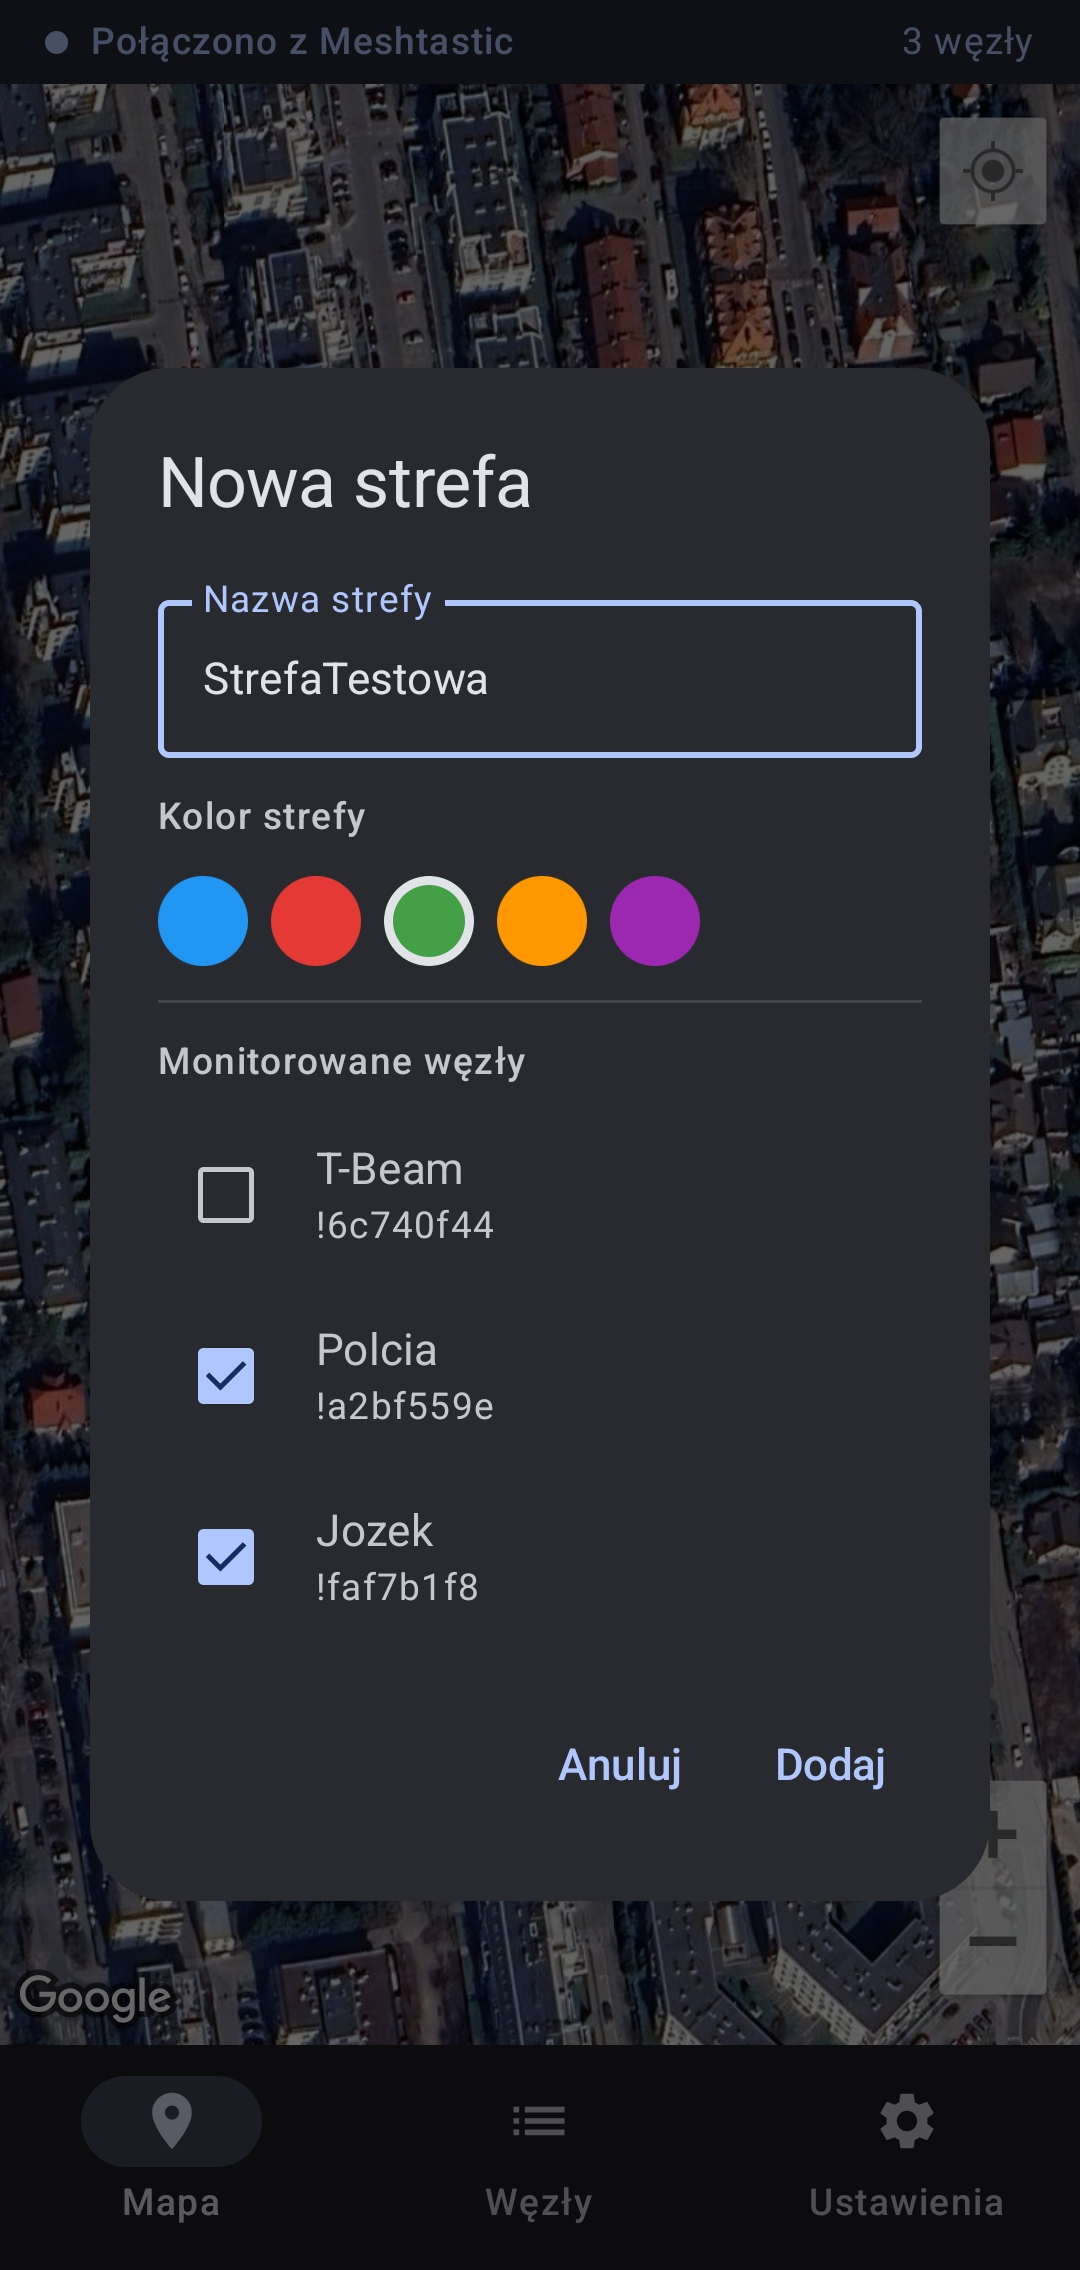
\includegraphics[width=\linewidth]{nowaStrefa.jpg}
        \caption{Formularz tworzenia nowej strefy}
        \label{fig:nowa-strefa}
    \end{subfigure}
    \hfill
    \begin{subfigure}{0.45\linewidth}
        \centering
        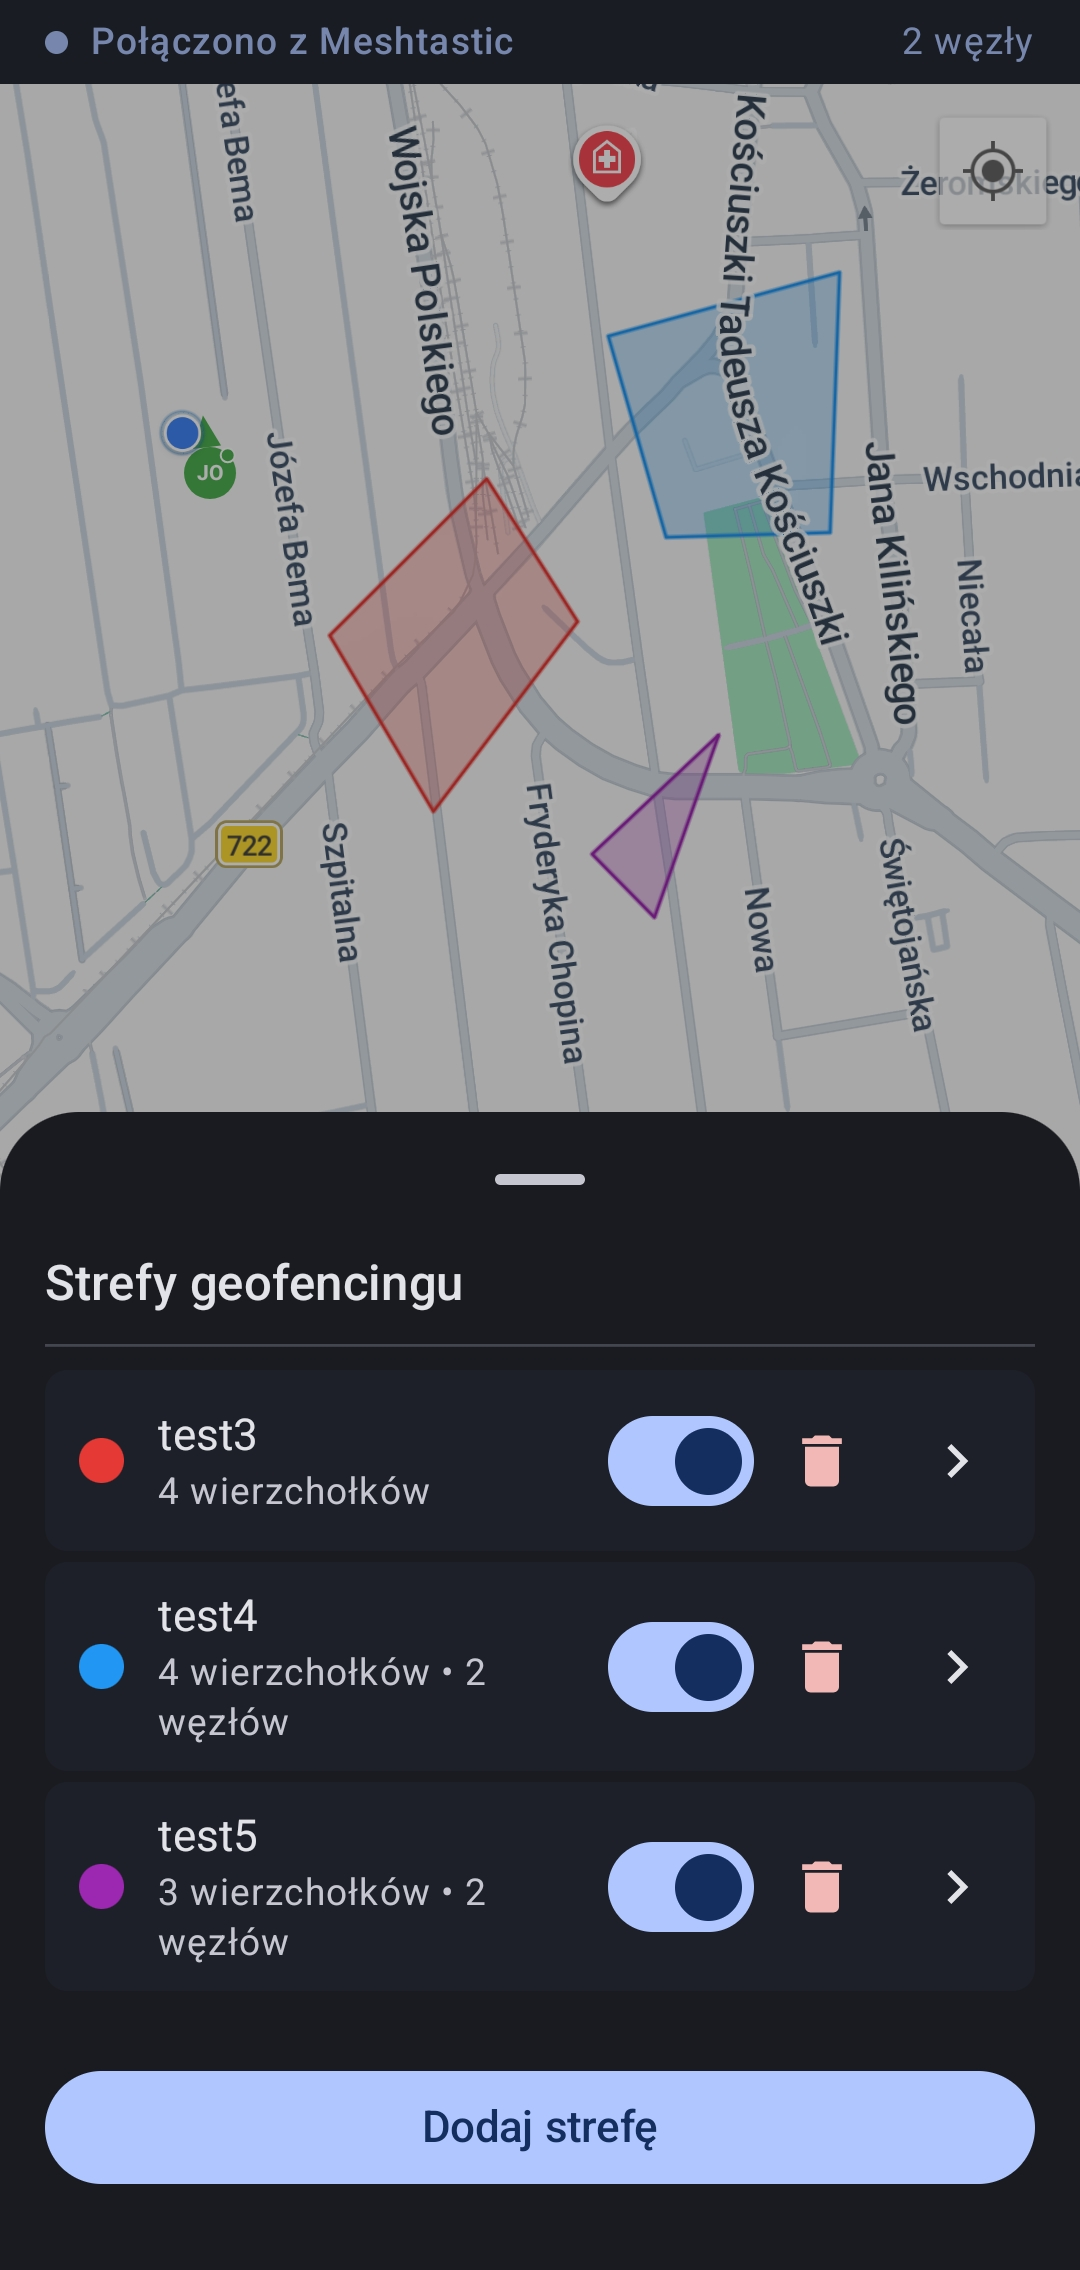
\includegraphics[width=\linewidth]{strefyLista.jpg}
        \caption{Lista zdefiniowanych stref}
        \label{fig:strefy-lista}
    \end{subfigure}
    \caption{Zarządzanie strefami geofencingu}
    \label{fig:geofencing-zarzadzanie}
\end{figure}

\paragraph{Węzły.}

Ekran listy węzłów (\texttt{NodeListScreen}) prezentuje wszystkie aktywne węzły wykryte
w sieci Meshtastic. Dla każdego węzła wyświetlane są jego nazwa, rola, czas ostatniej
aktywności oraz wskaźnik jakości sygnału (SNR) i RSSI\footnote{RSSI (ang.\
\textit{Received Signal Strength Indicator}) - bezwzględna moc odebranego sygnału,
wyrażona w~dBm. W odróżnieniu od SNR nie uwzględnia poziomu szumu, lecz informuje
o sile sygnału w punkcie odbioru.}. Lista może być filtrowana i sortowana,
co ułatwia odnalezienie konkretnego urządzenia w większej sieci. Dotknięcie węzła
otwiera ekran szczegółów (\texttt{NodeDetailScreen}), prezentujący pełne dane
telemetryczne - w tym poziom naładowania baterii, dokładne współrzędne GPS
oraz historię pozycji z bieżącej sesji w uproszczonej formie graficznej (rysunek~\ref{fig:wezly-lista}).

\paragraph{Ustawienia.}

Ekran ustawień (\texttt{SettingsScreen}) umożliwia konfigurację połączenia z aplikacją
Meshtastic. Użytkownik może tu wybrać urządzenie Bluetooth, z którym aplikacja ma się
połączyć, oraz monitorować aktualny stan połączenia. Ekran jest celowo minimalistyczny -
zgodnie z założeniem projektowym, konfiguracja powinna być jednorazowa i nie wymagać
powracania do ustawień podczas normalnej eksploatacji systemu.

\subsection*{Integracja z aplikacją Meshtastic}
\label{sec:integracja-meshtastic}

Aplikacja MeshTracker nie komunikuje się bezpośrednio z urządzeniami radiowymi - korzysta
z aplikacji Meshtastic zainstalowanej na tym samym telefonie, która pełni rolę pośrednika. 
Wybrano takie podejście, aby nie musieć implementować protokołu Meshtastic i skupić się na 
warstwie prezentacji i funkcjonalności geofencingu. 

\paragraph{Mechanizmy IPC.}

Meshtastic udpostępnia dwa mechanizmy IPC (ang.\ \textit{Inter-Process Communication}):

\begin{itemize}
    \item \textbf{Interfejs AIDL} (ang.\ \textit{Android Interface Definition Language}) -
          umożliwia synchroniczne wywołania metod na działającym serwisie, takie jak pobranie
          listy węzłów czy zapytanie o stan połączenia. MeshTracker korzysta z niego na żądanie,
          głównie przy inicjalizacji i cyklicznym odświeżaniu. \footnote{Na Androidzie jeden proces 
          nie może normalnie uzyskać dostępu do pamięci innego procesu. Aby się komunikować, muszą 
          rozkładać obiekty na elementy, które system operacyjny może zrozumieć, i przekazywać je 
          przez tę granicę. Kod potrzebny do tego przekształcania jest trudny do napisania, dlatego 
          Android wykonuje to za Ciebie za pomocą AIDL.[\url{https://developer.android.com/develop/background-work/services/aidl?hl=pl}]}

    \item \textbf{Broadcasty Androida} - Meshtastic rozsyła komunikaty do wszystkich
          zainteresowanych aplikacji przy każdej zmianie stanu sieci. Pozwala to na reaktywne
          powiadamianie o nowych danych bez aktywnego odpytywania serwisu.  
        \footnote{Aplikacje Androida mogą wysyłać i odbierać komunikaty systemowe oraz pochodzące z innych aplikacji, zgodnie ze wzorem projektowym \textit{publish-subscribe}. \url{https://developer.android.com/guide/components/broadcasts?hl=pl}}
\end{itemize}

MeshTracker korzysta z obu mechanizmów jednocześnie: AIDL do inicjalizacji stanu i cyklicznego
odświeżania, broadcasty do aktualizacji w czasie rzeczywistym. Gwarantuje to
spójność danych niezależnie od tego, czy zdarzenie nastąpi między cyklami odświeżania, czy
podczas startu aplikacji.

Takie podejście do integracji między aplikacjami wprowadza pewną wrażliwość na zmiany API Meshtastic między wersjami.
W szczególności metoda zwracająca ID węzła lokalnego zmieniała swoją nazwę w kolejnych
wydaniach, co wymagało zaimplementowania łańcucha kandydatów:
\texttt{getMyId()} $\to$ \texttt{getMyNodeId()} $\to$ \texttt{myId()} $\to$ \texttt{getOwnerId()}
$\to$ przez \texttt{\seqsplit{getMyNodeInfo().myNodeNum}}. Wersja Meshtastic na telefonie użytkownika
jest poza kontrolą dewelopera MeshTrackera, dlatego integracja musi być możliwie elastyczna i odporna na zmiany w API Meshtastic.

\subsection*{Schemat nawiązywania połączenia.}

Rysunek~\ref{fig:connection-flow} przedstawia sekwencję zdarzeń od uruchomienia
\texttt{MapViewModel} do pojawienia się węzła na mapie.

\begin{figure}[!h]
    \label{fig:connection-flow}
    \centering
    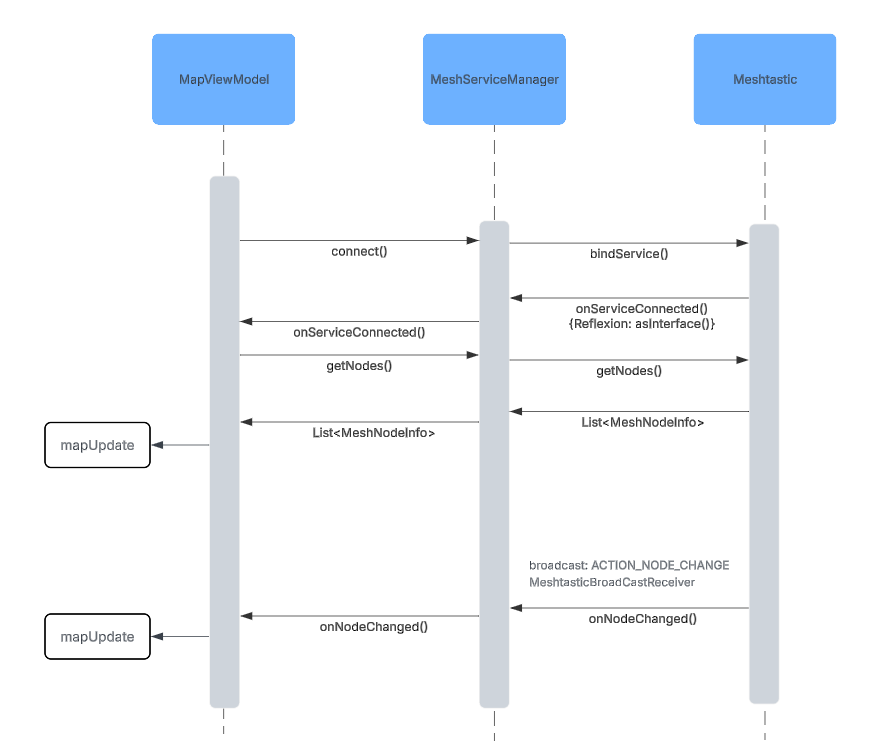
\includegraphics[width=\linewidth]{schematPolaczenia.png}
    \caption{Sekwencja nawiązywania połączenia i przepływ danych}
\end{figure}

\paragraph{Obsługa rozłączenia i błędów.}

Wyróżnione są dwa odrębne scenariusze rozłączenia, które wymagają różnej reakcji aplikacji:

\textbf{Rozłączenie celowe} następuje, gdy użytkownik zamyka aplikację. W \texttt{\seqsplit{MeshServiceManager}} flaga
\texttt{\seqsplit{isIntentionalDisconnect}} jest ustawiana przed wywołaniem \texttt{unbindService()}.
Gdy wywołana jest metoda \texttt{onServiceDisconnected()}, wartość powyższej flagi pozwala
pominąć propagację zdarzenia do warstwy UI, przez co użytkownik nie powinien widzieć komunikatu
o błędzie, skoro rozłączenie było planowane.

\textbf{Rozłączenie nieoczekiwane} - sygnalizuje, że serwis Meshtastic zakończył
działanie bez polecenia MeshTrackera (np.\ na skutek wymuszonego zamknięcia przez system).
W takim przypadku zdarzenie jest propagowane do \texttt{MapViewModel}, który aktualizuje
pasek stanu aplikacji (\texttt{\seqsplit{ConnectionStatusBar}}) odpowiednim komunikatem.

\paragraph{Automatyczna próba ponownego połączenia.}

Odebranie broadcastu \texttt{\seqsplit{ACTION\_MESH\_DISCONNECTED}} \footnote{Broadcasty nie są dostępne w dokumentacji API, jednak można je znaleźć dobrze udokumentowane w repozytorium \url{https://github.com/meshtastic/Meshtastic-Android/blob/main/core/api/src/main/kotlin/org/meshtastic/core/api/MeshtasticIntent.kt}} przy wciąż aktywnym bindingu
z serwisem (tj.\ gdy \texttt{isBound~=~true}) uruchamia w \texttt{\seqsplit{MapViewModel}} procedurę
automatycznego wznawiania połączenia z węzłem lokalnym (\texttt{startReconnecting()}). Działa ona
w pętli, która wykonywana jest aż do skutku lub utraty samego bindingu.

Każda iteracja pętli rozpoczyna się odliczaniem \texttt{\seqsplit{RECONNECT\_INTERVAL\_SECONDS}}~=~30
sekund. W tym czasie stan połączenia ustawiany jest na \texttt{\seqsplit{ConnectionState.Reconnecting}},
który przechowuje liczbę sekund pozostałych do następnej próby. Wartość ta jest co sekundę
odświeżana i wyświetlana użytkownikowi w pasku stanu \texttt{\seqsplit{ConnectionStatusBar}}, dzięki czemu
wie on, kiedy spodziewać się kolejnej próby.

Po upływie odliczania \texttt{MapViewModel} odpytuje serwis przez AIDL o aktualny stan połączenia z węzłem lokalnym.
Jeśli zwrócona wartość to \texttt{STATE\_CONNECTED}, procedura kończy działanie, a aplikacja
przechodzi w stan \texttt{Connected} i wznawia cykliczne odświeżanie węzłów. W przeciwnym razie
licznik prób jest inkrementowany i odliczanie zaczyna się od nowa. Jeśli podczas oczekiwania
binding z serwisem zostanie utracony (\texttt{isConnected()~=~false}), pętla jest przerywana,
a stan przechodzi w \texttt{Disconnected}.

Niezależnie od automatycznych prób, użytkownik może w dowolnej chwili nacisnąć przycisk
\textit{Ponów} widoczny w pasku stanu (rysunek~\ref{fig:connection-status}). Wywołuje to \texttt{retryConnect()},
które anuluje bieżące zadania, resetuje binding i inicjuje nowe połączenie z serwisem
od zera. Jest to przydatne np. gdy użytkownik ręcznie uruchomił aplikację Meshtastic i chce wywołać
natychmiastową próbę połączenia bez czekania na automatyczne odświeżenie.

\begin{figure}[H]
\centering
\begin{tikzpicture}[
    node distance=0.7cm,
    every node/.style={font=\small},
    io/.style={ellipse, draw=black, fill=gray!18,
        text width=4.2cm, minimum height=0.72cm, align=center},
    proc/.style={rectangle, draw=black, fill=blue!7,
        text width=4.2cm, minimum height=0.72cm, align=center},
    dec/.style={diamond, draw=black, fill=orange!15,
        minimum width=3.2cm, minimum height=1.0cm,
        align=center, inner sep=1pt},
    endok/.style={ellipse, draw=black, fill=green!15,
        text width=3.6cm, minimum height=0.72cm, align=center},
    enderr/.style={ellipse, draw=black, fill=red!10,
        text width=3.2cm, minimum height=0.72cm, align=center},
    side/.style={rectangle, draw=black!50, dashed, fill=yellow!10,
        text width=3.5cm, minimum height=0.72cm, align=center},
    arr/.style={->, >=Stealth, thick},
    darr/.style={->, >=Stealth, thick, dashed},
    lbl/.style={font=\scriptsize},
]
% Główny przepływ
\node[io] (recv)  {\small Odebranie \texttt{\seqsplit{ACTION\_MESH\_DISCONNECTED}}\\[1pt]
                   {\scriptsize\texttt{isBound = true}}};
\node[proc,  below=of recv]       (startR) {\texttt{startReconnecting()}};
\node[proc,  below=of startR]     (setR)   {Stan $\to$ \texttt{Reconnecting}};
\node[proc,  below=of setR]       (waitN)  {Odczekaj 30\,s\\[1pt]
                                             {\scriptsize aktualizuj UI co 1\,s}};
\node[dec,   below=0.9cm of waitN] (decB)  {Binding\\utracony?};
\node[proc,  below=0.9cm of decB]  (aidlQ) {Zapytaj serwis AIDL\\[1pt]
                                             o stan połączenia};
\node[dec,   below=0.9cm of aidlQ] (decC)  {\texttt{STATE\_}\\[-1pt]\texttt{CONNECTED?}};
\node[proc,  below=0.9cm of decC]  (incr)  {Inkrementuj\\licznik prób};

% Stany końcowe (prawa kolumna)
\node[enderr, right=2.6cm of decB] (disc) {Stan $\to$ \texttt{Disconnected}};
\node[endok,  right=2.6cm of decC] (conn) {Stan $\to$ \texttt{Connected}\\[1pt]
                                            {\scriptsize wznów odświeżanie}};

% Ścieżka użytkownika (prawa kolumna, u góry)
\node[side, right=2.6cm of startR]  (ponow)   {Użytkownik:\\przycisk ,,Ponów''};
\node[side, below=0.6cm of ponow]   (retryFn) {\texttt{retryConnect()}\\[1pt]
                                               {\scriptsize anuluj, reset bindingu}};

% Strzałki głównego przepływu
\draw[arr] (recv)  -- (startR);
\draw[arr] (startR)-- (setR);
\draw[arr] (setR)  -- (waitN);
\draw[arr] (waitN) -- (decB);
\draw[arr] (decB)  -- node[lbl, above] {Tak} (disc);
\draw[arr] (decB)  -- node[lbl, left=2pt] {Nie} (aidlQ);
\draw[arr] (aidlQ) -- (decC);
\draw[arr] (decC)  -- node[lbl, above] {Tak} (conn);
\draw[arr] (decC)  -- node[lbl, left=2pt] {Nie} (incr);

% Pętla powrotna (lewa strona)
\draw[arr] (incr.west) -- ++(-1.8,0) |- (setR.west);

% Ścieżka przycisku "Ponów"
\draw[darr] (ponow)   -- (retryFn);
\draw[darr] (retryFn) to[bend right=45] (startR.east);
\end{tikzpicture}
\caption{Procedura automatycznego ponownego połączenia}
\label{fig:reconnect-flow}
\end{figure}

\begin{figure}[!h]
    \label{fig:connection-status}
    \centering
    
\includegraphics[width=0.45\linewidth]{nieMoznaPolaczycPasek.jpg}
    \caption{Pasek stanu połączenia - \textit{Ponów}}
\end{figure}

\paragraph{Model danych węzła.}

Obiekt \texttt{NodeInfo} udostępniany przez Meshtastic jest mapowany na wewnętrzną strukturę
danych złożoną z trzech klas: \texttt{MeshNodeInfo}, \texttt{MeshUserInfo} oraz
\texttt{MeshPosition}. 

Klasa \texttt{MeshNodeInfo} przechowuje dane identyfikacyjne i~telemetryczne węzła
(tabela~\ref{tab:meshnodeinfo}).

\begin{table}[!h]
    \caption{Pola klasy \texttt{MeshNodeInfo}}
    \label{tab:meshnodeinfo}
    \centering
    \begin{tabular}{|l|l|p{6.5cm}|}
        \hline
        \textbf{Pole} & \textbf{Typ} & \textbf{Opis} \\
        \hline
        \texttt{num}          & \texttt{Int}           & Unikalny numer węzła w sieci Meshtastic \\
        \texttt{user}         & \texttt{MeshUserInfo} & Dane użytkownika węzła (nazwa, rola, sprzęt) \\
        \texttt{position}     & \texttt{MeshPosition} & Ostatnia znana pozycja GPS \\
        \texttt{snr}          & \texttt{Float}         & SNR ostatnio odebranego pakietu [dB] \\
        \texttt{rssi}         & \texttt{Int}           & RSSI ostatnio odebranego pakietu [dBm] \\
        \texttt{lastHeard}    & \texttt{Int}           & Czas ostatniego odbioru (Unix timestamp [s]) \\
        \texttt{batteryLevel} & \texttt{Int}           & Poziom naładowania baterii [\%] \\
        \texttt{channel}      & \texttt{Int}           & Indeks kanału, na którym węzeł nadaje \\
        \texttt{hopsAway}     & \texttt{Int}           & Liczba przeskoków do węzła w sieci mesh \\
        \hline
    \end{tabular}
\end{table}

Klasa \texttt{MeshUserInfo} zawiera dane konfiguracyjne przypisane do węzła przez jego
właściciela (tabela~\ref{tab:meshuserinfo}).

\begin{table}[!h]
    \caption{Pola klasy \texttt{MeshUserInfo}}
    \label{tab:meshuserinfo}
    \centering
    \begin{tabular}{|l|l|p{6.5cm}|}
        \hline
        \textbf{Pole} & \textbf{Typ} & \textbf{Opis} \\
        \hline
        \texttt{id}            & \texttt{String}  & Identyfikator w formacie \texttt{!XXXXXXXX} \\
        \texttt{longName}      & \texttt{String}  & Pełna nazwa węzła nadana przez użytkownika \\
        \texttt{shortName}     & \texttt{String}  & Skrócona nazwa (do 4 znaków), widoczna na wyświetlaczu węzła \\
        \texttt{hwModelString} & \texttt{String} & Model sprzętu (np.\ \texttt{T\_BEAM}, \texttt{T\_ECHO}, \texttt{T1000\_E}) \\
        \texttt{isLicensed}    & \texttt{Boolean} & Czy węzeł jest zarejestrowany jako amatorska stacja radiowa \\
        \texttt{role}          & \texttt{Int}     & Rola węzła w sieci (CLIENT, ROUTER, TRACKER itp.) \\
        \hline
    \end{tabular}
\end{table}

Klasa \texttt{MeshPosition} przechowuje dane lokalizacyjne węzła
(tabela~\ref{tab:meshposition}). Warto zwrócić uwagę na dwie nieoczywiste konwencje
kodowania stosowane przez Meshtastic: współrzędne geograficzne przechowywane są jako liczby
całkowite (w formacie stopni pomnożonych przez $10^7$) 
\footnote{\url{https://github.com/meshtastic/Meshtastic-Android/blob/19ea164f93bd48dd556d5232d66869b5cb0b2f40/core/model/src/commonMain/kotlin/org/meshtastic/core/model/Node.kt\#L110}} ,
co pozwala na precyzję nawet do około 1 metra bez użycia typów zmiennoprzecinkowych. Natomiast kierunek ruchu (\texttt{groundTrack}) wyrażony jest, z podobnej przyczyny, w setnych stopniach (pomnożonych przez $10^5$).

\begin{table}[!h]
    \caption{Pola klasy \texttt{MeshPosition}}
    \label{tab:meshposition}
    \centering
    \begin{tabular}{|l|l|p{6.5cm}|}
        \hline
        \textbf{Pole} & \textbf{Typ} & \textbf{Opis} \\
        \hline
        \texttt{latitude}        & \texttt{Double} & Szerokość geograficzna [${}^\circ$], po konwersji z $10^7$ \\
        \texttt{longitude}       & \texttt{Double} & Długość geograficzna [${}^\circ$], po konwersji z $10^7$ \\
        \texttt{altitude}        & \texttt{Int}    & Wysokość [m n.p.m.] \\
        \texttt{time}            & \texttt{Int}    & Unix timestamp [s] \\
        \texttt{satellitesInView}& \texttt{Int}    & Liczba widocznych satelitów \\
        \texttt{groundSpeed}     & \texttt{Int}    & Prędkość [m/s] \\
        \texttt{groundTrack}     & \texttt{Int}    & Kierunek ruchu [${}^\circ$](0\,=\,N) \\
        \texttt{precisionBits}   & \texttt{Int}    & Precyzja pozycji (liczba bitów, max 32\,$\approx$\,1\,m) \\
        \hline
    \end{tabular}
\end{table}

Dostępność poszczególnych pól pozycji zależy od konfiguracji węzła nadającego, a konkretnie
od wartości \textit{Position Flags}, czyli bitowego pola opcji włączanych w ustawieniach
radia Meshtastic.\footnote{\url{https://meshtastic.org/docs/configuration/radio/position/\#position-config-values}}
Tabela~\ref{tab:position-flags} zestawia dostępne flagi.

\begin{table}[!h]
    \caption{Flagi \textit{Position Flags} - pola opcjonalne pakietu pozycji}
    \label{tab:position-flags}
    \centering
    \begin{tabular}{|l|p{9cm}|}
        \hline
        \textbf{Flaga} & \textbf{Opis} \\
        \hline
        \texttt{ALTITUDE}           & Dołącza wartość wysokości (jeśli dostępna) \\
        \texttt{ALTITUDE\_MSL}      & Wysokość wyrażona jako MSL (nad poziomem morza) \\
        \texttt{GEOIDAL\_SEPARATION}& Dołącza separację geoidy\footnotemark \\
        \texttt{DOP}                & Dołącza wskaźnik DOP (domyślnie PDOP)\footnotemark{} \\
        \texttt{HVDOP}              & Zamiast PDOP wysyła osobne wartości HDOP i VDOP\footnotemark \\
        \texttt{SATINVIEW}          & Dołącza liczbę widocznych satelitów \\
        \texttt{SEQ\_NO}            & Dołącza numer sekwencyjny pakietu (rośnie co pakiet) \\
        \texttt{TIMESTAMP}          & Dołącza znacznik czasu z rozwiązania GPS \\
        \texttt{HEADING}            & Dołącza kierunek ruchu z rozwiązania GPS \\
        \texttt{SPEED}              & Dołącza prędkość naziemną z rozwiązania GPS \\
        \hline
    \end{tabular}
\end{table}
\addtocounter{footnote}{-2}
\footnotetext{Separacja geoidy (ang.\ \textit{geoidal separation}) to różnica wysokości między
elipsoidą odniesienia (np.\ WGS-84) a geoidą -- powierzchnią ekwipotencjalną odpowiadającą
średniemu poziomowi morza. Niezbędna do przeliczenia wysokości elipsoidalnej GPS na wysokość
nad poziomem morza (MSL).}
\addtocounter{footnote}{1}
\footnotetext{DOP (ang.\ \textit{Dilution of Precision}) to bezwymiarowy wskaźnik jakości geometrii
konstelacji satelitów widocznych w danej chwili. PDOP (ang.\ \textit{Position DOP}) opisuje łączną
precyzję wyznaczania pozycji 3D. Im mniejsza wartość, tym lepsza geometria konstelacji satelitów.}
\addtocounter{footnote}{1}
\footnotetext{HDOP (ang.\ \textit{Horizontal Dilution of Precision}) -- wskaźnik precyzji wyznaczania
pozycji w płaszczyźnie poziomej; VDOP (ang.\ \textit{Vertical Dilution of Precision}) -- analogiczny
wskaźnik dla składowej pionowej.}

W konfiguracji przyjętej w projekcie włączone są flagi \texttt{\seqsplit{ALTITUDE}}, \texttt{\seqsplit{SATINVIEW}},
\texttt{\seqsplit{TIMESTAMP}}, \texttt{\seqsplit{HEADING}} oraz \texttt{\seqsplit{SPEED}}. Flagi są ustawiane per węzeł nadający.
Precyzja ustalania pozycji ustalana jest na poziomie kanału. Ustawiono  maksymalną możliwą 
wartość - 32-bity na kanale \texttt{Reja} Jeśli dane pole nie jest aktywowane, w odebranym 
pakiecie przyjmuje wartość domyślną (zwykle 0), co MeshTracker traktuje jako brak danych. 



\subsection*{Geofencing}
\label{sec:geofencing}

Geofencing polega na wykrywaniu przekroczenia przez obiekt wirtualnej granicy
geograficznej wyłącznie w oparciu o dane lokalizacyjne. Ostatecznie projekt ma na celu,
żeby użytkownik dostał powiadomienie w momencie, gdy węzeł przekroczy granicę wyznaczonego 
obszaru. W projekcie MeshTracker granice definiowane są jako wielokąty o dowolnym kształcie.

\subsection*{Model danych.}

Dane geofencingu przechowywane są w bazie Room za pomocą dwóch encji:
\texttt{Zone} i~\texttt{ZoneEvent} (tabele~\ref{tab:zone-entity}
i~\ref{tab:zoneevent-entity}).

\begin{table}[!h]
    \caption{Encja \texttt{Zone} - strefa geofencingu}
    \label{tab:zone-entity}
    \centering
    \begin{tabular}{|l|l|p{7cm}|}
        \hline
        \textbf{Pole} & \textbf{Typ} & \textbf{Opis} \\
        \hline
        \texttt{id}                 & \texttt{String (UUID)} & Klucz główny, generowany jako UUID v4 \\
        \texttt{name}               & \texttt{String}        & Nazwa nadana przez użytkownika \\
        \texttt{colorArgb}          & \texttt{Int}           & Kolor strefy (ARGB\footnote{ARGB - format kodowania koloru jako 32-bitowa liczba całkowita złożona z czterech 8-bitowych kanałów: Alpha (przezroczystość), Red, Green, Blue.} packed Int) \\
        \texttt{isActive}           & \texttt{Boolean}       & Czy strefa jest aktywnie monitorowana \\
        \texttt{verticesJson}       & \texttt{String}        & Wierzchołki wielokąta w formacie JSON \\
        \texttt{watchedNodeIdsJson} & \texttt{String}        & Lista ID węzłów do monitorowania w JSON \\
        \hline
    \end{tabular}
\end{table}

Wierzchołki wielokąta i lista monitorowanych węzłów przechowywane są jako serializowane
tablice JSON, przykładowo: \texttt{[\{"lat":52.1,"lon":21.0\},\ldots]}.

\begin{table}[!h]
    \caption{Encja \texttt{ZoneEvent} - zdarzenie wejścia/wyjścia ze strefy}
    \label{tab:zoneevent-entity}
    \centering
    \small
    \begin{tabular}{|p{2.8cm}|p{2.6cm}|p{6.5cm}|}
        \hline
        \textbf{Pole} & \textbf{Typ} & \textbf{Opis} \\
        \hline
        \texttt{id}               & \texttt{Long} (autoincrement) & Klucz główny \\
        \texttt{zoneId}           & \texttt{String}               & ID strefy  \\
        \texttt{nodeId}           & \texttt{String}               & ID węzła w chwili zdarzenia \\
        \texttt{eventType}        & \texttt{String}               & \texttt{"ENTER"} lub \texttt{"EXIT"} \\
        \texttt{\seqsplit{timestampSeconds}} & \texttt{Int}                  & Czas zdarzenia (Unix timestamp [s]) \\
        \hline
    \end{tabular}
    \normalsize
\end{table}


\paragraph{Algorytm sprawdzania przynależności do strefy.}

Do wykrywania, czy punkt GPS leży wewnątrz wielokąta strefy, zastosowano algorytm
\textbf{rzucania promienia} (ang.\ \textit{ray casting}) \footnote{\url{https://www.geeksforgeeks.org/cpp/point-in-polygon-in-cpp/}}.
Jest to jeden z~najszerzej stosowanych algorytmów rozwiązujących problem PIP (ang.\
\textit{Point-In-Polygon}) ze względu na prostotę implementacji i niską złożoność obliczeniową
$O(n)$, gdzie $n$ to liczba wierzchołków wielokąta~\cite{shimrat1962}. Uzasadnienie wyboru
akurat tej metody, oraz omówienie rozwiązań alternatywnych, zamieszczono na końcu rozdz.~\ref{sec:geofencing}.

Zasada działania jest następująca (rysunek~\ref{fig:ray-casting}). Z badanego punktu $P = (x_P, y_P)$
wysyłany jest poziomy promień w kierunku rosnącej długości geograficznej $y \to +\infty$.
Zliczana jest liczba przecięć promienia z krawędziami wielokąta:

\begin{itemize}
    \item nieparzysta liczba przecięć $\Rightarrow$ punkt leży \textbf{wewnątrz} wielokąta,
    \item parzysta liczba przecięć $\Rightarrow$ punkt leży \textbf{na zewnątrz}.
\end{itemize}

Dla każdej krawędzi łączącej wierzchołki $X_i = (x_i, y_i)$
i~$Y_j = (x_j, y_j)$ sprawdzany jest warunek przecięcia z promieniem:
krawędź musi mieć jeden wierzchołek ściśle powyżej szerokości geograficznej punktu
$x_P$, a drugi poniżej lub równo z nią. Jeśli warunek jest spełniony, wyznaczana jest
długość geograficzna przecięcia:

\begin{equation}
    y_{\text{przecięcia}} = y_i +
        \frac{x_P - x_i}{x_j - x_i} \cdot (y_j - y_i)
    \label{eq:ray-cast-cross}
\end{equation}

Przecięcie jest liczone tylko jeśli $y_P < y_{\text{przecięcia}}$, tzn.\ leży
na prawo od badanego punktu (promień biegnie w prawo). Każde takie przecięcie neguje
bieżącą wartość flagi \texttt{inside}, która na początku wynosi \texttt{false}.

\begin{figure}[!h]
    \label{fig:ray-casting}
    \centering
    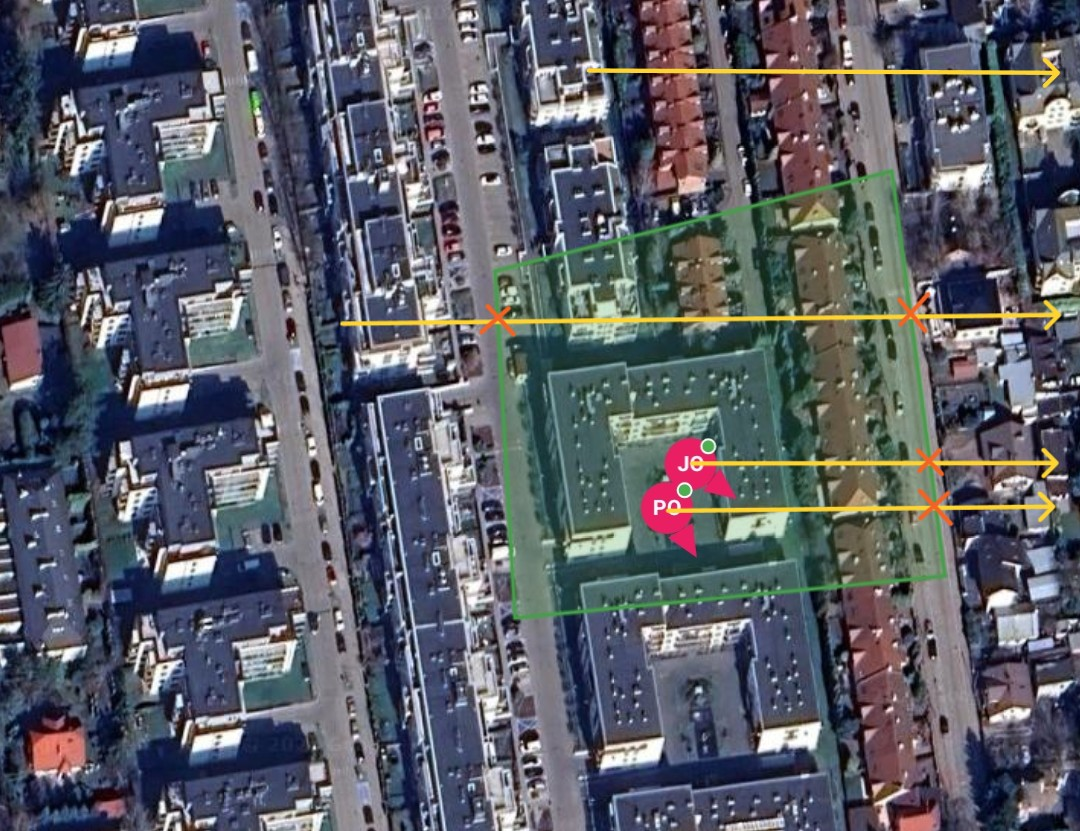
\includegraphics[width=\linewidth]{strefaGeofencingRayCasting.jpg}
    \caption{Wizualizacja algorytmu ray casting - liczba punktów przecięcia z krawędziami jednoznacznie wskazuje, czy punkt leży wewnątrz czy na zewnątrz wielokąta}
\end{figure}


\begin{lstlisting}[caption={Implementacja algorytmu ray casting w \texttt{GeofenceChecker.contains()}},
                   label={lst:geofence-contains},
                   basicstyle=\footnotesize\ttfamily,
                   xleftmargin=0pt]
fun contains(
    pointLat: Double,
    pointLon: Double,
    polygon: List<ZoneVertex>
): Boolean {
    if (polygon.size < 3) return false

    var inside = false
    var j = polygon.lastIndex

    for (i in polygon.indices) {
        val vi = polygon[i]
        val vj = polygon[j]

        // Czy krawedz przecina poziomy promien z punktu w prawo?
        val crossesRay =
            (vi.lat <= pointLat && vj.lat > pointLat) ||
            (vj.lat <= pointLat && vi.lat > pointLat)

        if (crossesRay) {
            // Dlugosc geograficzna przeciecia promienia z krawedzia
            val intersectLon = vi.lon +
                (pointLat-vi.lat)/(vj.lat-vi.lat)*(vj.lon-vi.lon)

            if (pointLon < intersectLon) {
                inside = !inside
            }
        }
        j = i
    }
    return inside
}
\end{lstlisting}

Implementacja obsługuje wielokąty \emph{wklęsłe} i~\emph{wypukłe} oraz~\emph{złożone} (z przecięciami własnymi). 
Nie jest jednak zoptymalizowana pod kątem przypadków brzegowych, takich jak punkt leżący dokładnie na krawędzi 
lub wierzchołku wielokąta - w takich sytuacjach wynik może być nieprzewidywalny. W praktyce, ze względu na 
niedokładność GPS, takie przypadki są pomijalnie rzadkie i nie stanowią problemu dla funkcjonalności aplikacji.

\subsection*{Wykrywanie zdarzeń wejścia i wyjścia.}

Aby wygenerować zdarzenia \texttt{ENTER} i \texttt{EXIT}, konieczne jest śledzenie
zmian stanu między kolejnymi aktualizacjami pozycji.
\texttt{\seqsplit{ZoneMonitorService}} utrzymuje słownik \texttt{\seqsplit{previousNodeZoneMap}},
mapujący~ID~węzła na zbiór ID stref, w których węzeł znajdował się przy poprzedniej
aktualizacji. Po każdym odebraniu broadcastu \texttt{\seqsplit{ACTION\_NODE\_CHANGE}} wykonywane są trzy kroki:

\begin{enumerate}
    \item Obliczany jest zbiór stref \texttt{currentZones} zawierających węzeł
          w~chwili obecnej (tylko spośród stref, które ten węzeł monitorują).
    \item Zdarzenia \texttt{ENTER} generowane są dla stref obecnych w \texttt{currentZones},
          ale nieobecnych w \texttt{previousZones}.
    \item Zdarzenia \texttt{EXIT} generowane są dla stref obecnych w \texttt{previousZones},
          ale nieobecnych w \texttt{currentZones}.
\end{enumerate}

Po przetworzeniu słownik jest aktualizowany w taki sposób, że jeżeli węzeł nie znajduje się w~żadnej strefie,
jego wpis jest usuwany, co minimalizuje zużycie pamięci.

\paragraph{ZoneMonitorService - monitorowanie w tle.}

Logika geofencingu działa w ramach \texttt{ZoneMonitor\-Service} - usługi pierwszoplanowej
(ang.\ \textit{foreground service}) Androida. Jest to jedyna niezawodna metoda utrzymania
procesu aktywnego w tle: system Android agresywnie wstrzymuje zwykłe procesy w tle w celu
oszczędzania baterii, natomiast usługi pierwszoplanowe są przed tym chronione, pod warunkiem
że wyświetlają stałe powiadomienie systemowe~\cite{android-foreground-service}.

Cykl życia serwisu przebiega następująco:
\begin{itemize}
    \item \textbf{Uruchomienie}: \texttt{ZoneViewModel} wywołuje \texttt{ZoneMonitorService.start()},
          gdy w bazie danych istnieje \textbf{co najmniej jedna aktywna strefa}.
    \item \textbf{Działanie}: serwis rejestruje \texttt{MeshtasticBroadcastReceiver}
          i subskrybuje zmiany stref z bazy Room \footnote{Room to biblioteka Androida (część Jetpack) będąca warstwą abstrakcji nad SQLite. Zamiast pisać surowe zapytania SQL i ręcznie mapować wyniki na obiekty, definiuje się klasy encji (@Entity) i interfejsy DAO (@Dao) z adnotacjami, a Room generuje całą implementację w czasie kompilacji. W projekcie przechowuje strefy i log zdarzeń.} poprzez \texttt{Flow}\footnote{Flow to mechanizm z biblioteki Kotlin Coroutines reprezentujący asynchroniczny strumień wartości — analogia do LiveData, ale wbudowana w język. Room potrafi zwracać Flow<List<Zone>> zamiast jednorazowej listy: za każdym razem gdy dane w bazie się zmienią, Room automatycznie emituje nową listę do wszystkich subskrybentów. Właśnie dlatego zarówno ViewModel, jak i serwis są natychmiast powiadamiane o zmianach stref bez odpytywania bazy.}. Dzięki temu każda
          modyfikacja strefy jest propagowana do serwisu w czasie rzeczywistym, bez
          konieczności jego restartu.
    \item \textbf{Samozatrzymanie}: gdy \texttt{Flow} z Room zwróci pustą listę aktywnych
          stref (np.\ wszystkie zostały wyłączone lub usunięte), serwis wywołuje
          \texttt{stopSelf()} i kończy działanie autonomicznie.
    \item \textbf{Zatrzymanie zewnętrzne}: \texttt{ZoneViewModel} wywołuje
          \texttt{\seqsplit{ZoneMonitorService.stop()}} w reakcji na \textbf{wyłączenie ostatniej strefy}
          przez użytkownika.
\end{itemize}

\subsection*{Powiadomienia o przekroczeniu strefy.}

Wykrycie zdarzenia \texttt{ENTER} lub \texttt{EXIT} wyzwala wysłanie powiadomienia.
Powiadomienie zawiera nazwę węzła i nazwę strefy (rysunek~\ref{fig:strefa-powiadomienie-wejscia}), wysyłane jest z priorytetem \texttt{\seqsplit{PRIORITY\_HIGH}}
(kanał \texttt{\seqsplit{CHANNEL\_ZONE\_ALERTS}}) i~automatycznie znika po dotknięciu.
Przy pierwszym uruchomeniu aplikacji użytkownik musi jawnie przyznać
uprawnienie \texttt{\seqsplit{POST\_NOTIFICATIONS}}
(rysunek~\ref{fig:uprawnienia-powiadomienia}; obok lokalizacji i Bluetooth). Brak uprawnienia powoduje pominięcie powiadomienia bez
przerwania działania serwisu, co jest zachowaniem świadomym: serwis dalej wykrywa zdarzenia
i zapisuje je w bazie, jedynie nie wyświetla alertu.

\begin{figure}[!h]
    \centering
    \begin{minipage}{0.48\linewidth}
        \centering
        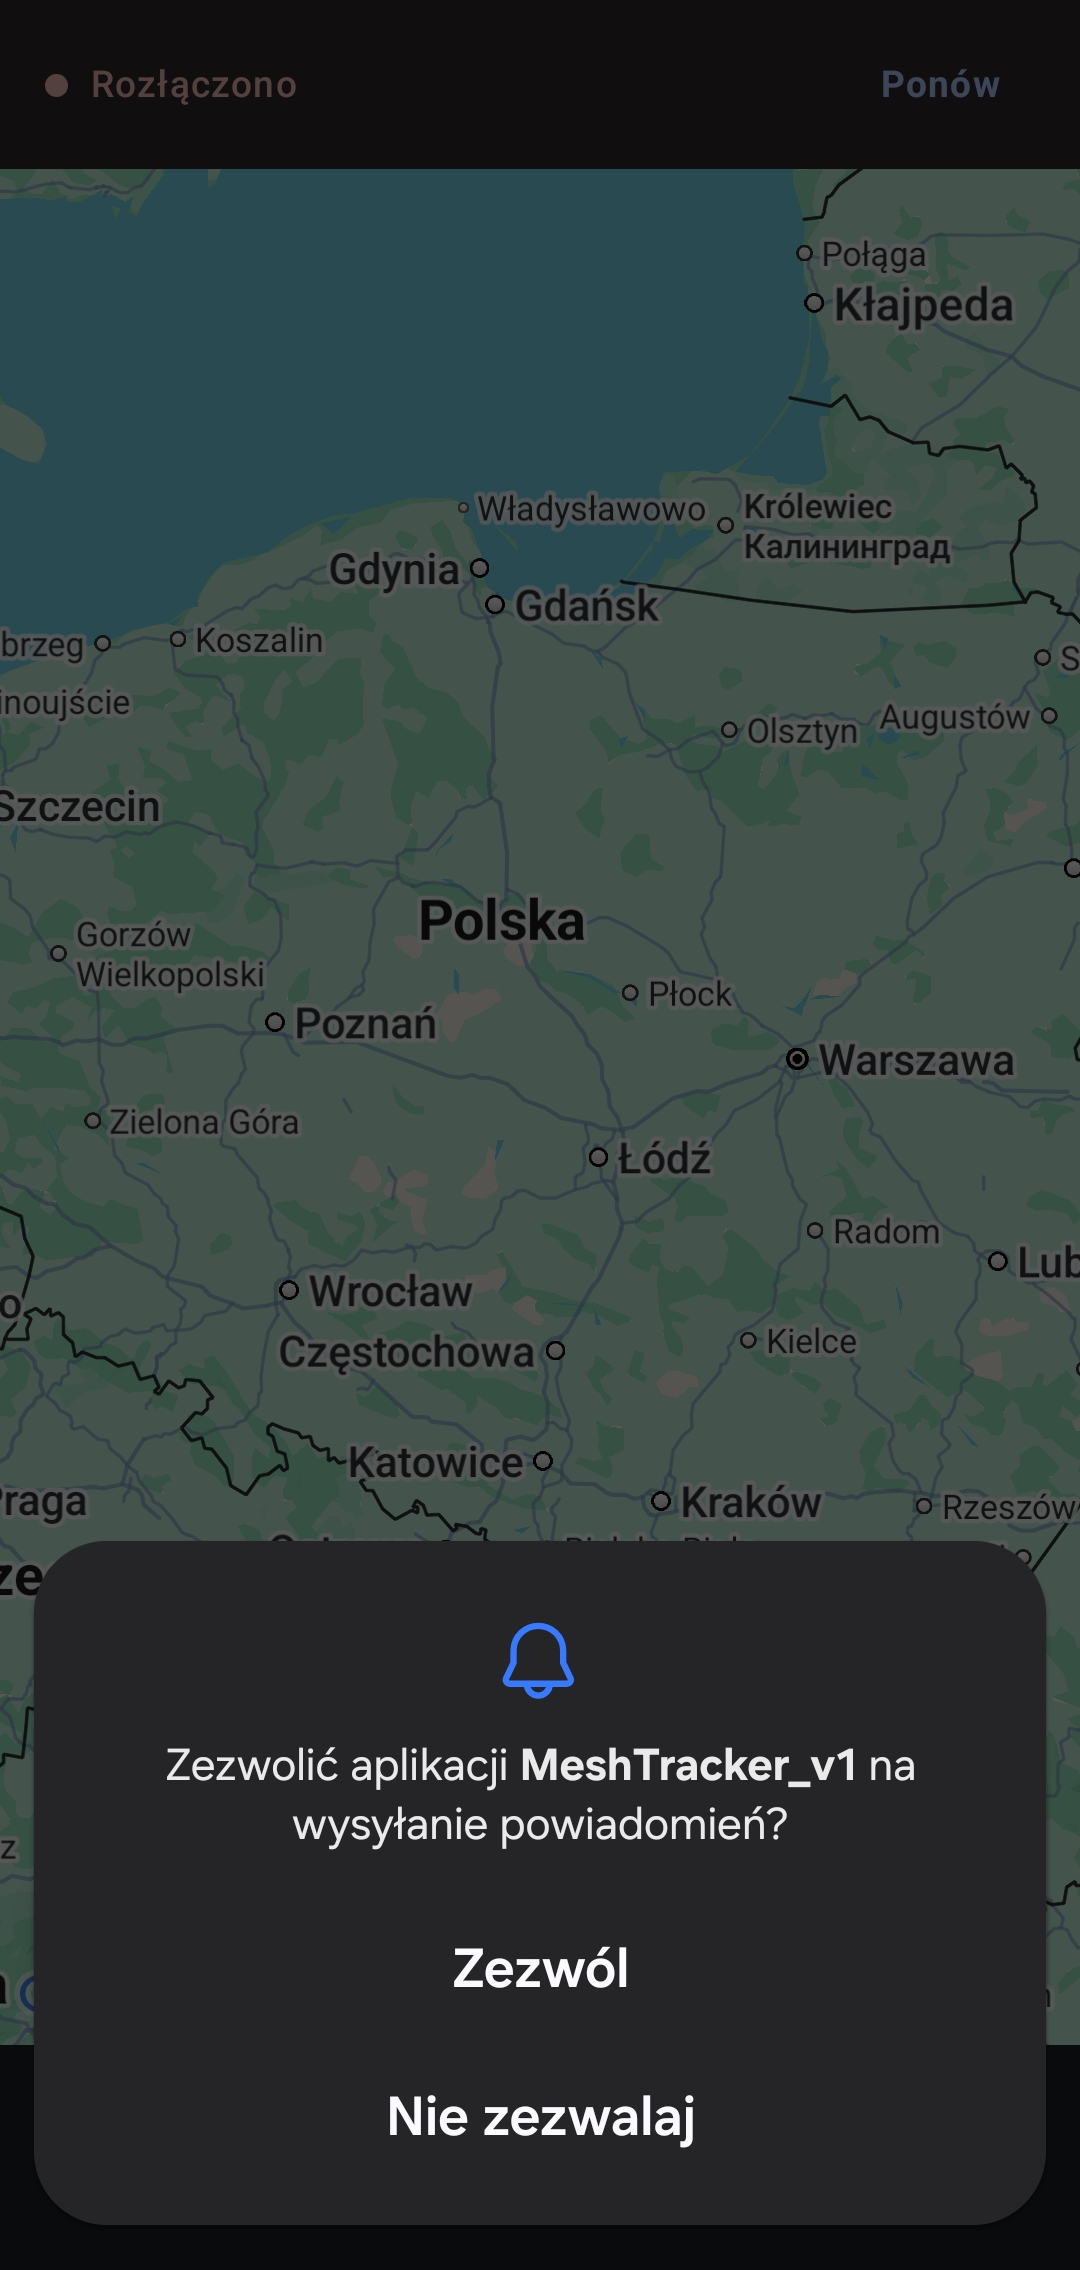
\includegraphics[width=\linewidth]{uprawnieniaPowiadomienia.jpg}
        \caption{Prośba o uprawnienie - \texttt{POST\_NOTIFICATIONS}}
        \label{fig:uprawnienia-powiadomienia}
    \end{minipage}
    \hfill
    \begin{minipage}{0.48\linewidth}
        \centering
        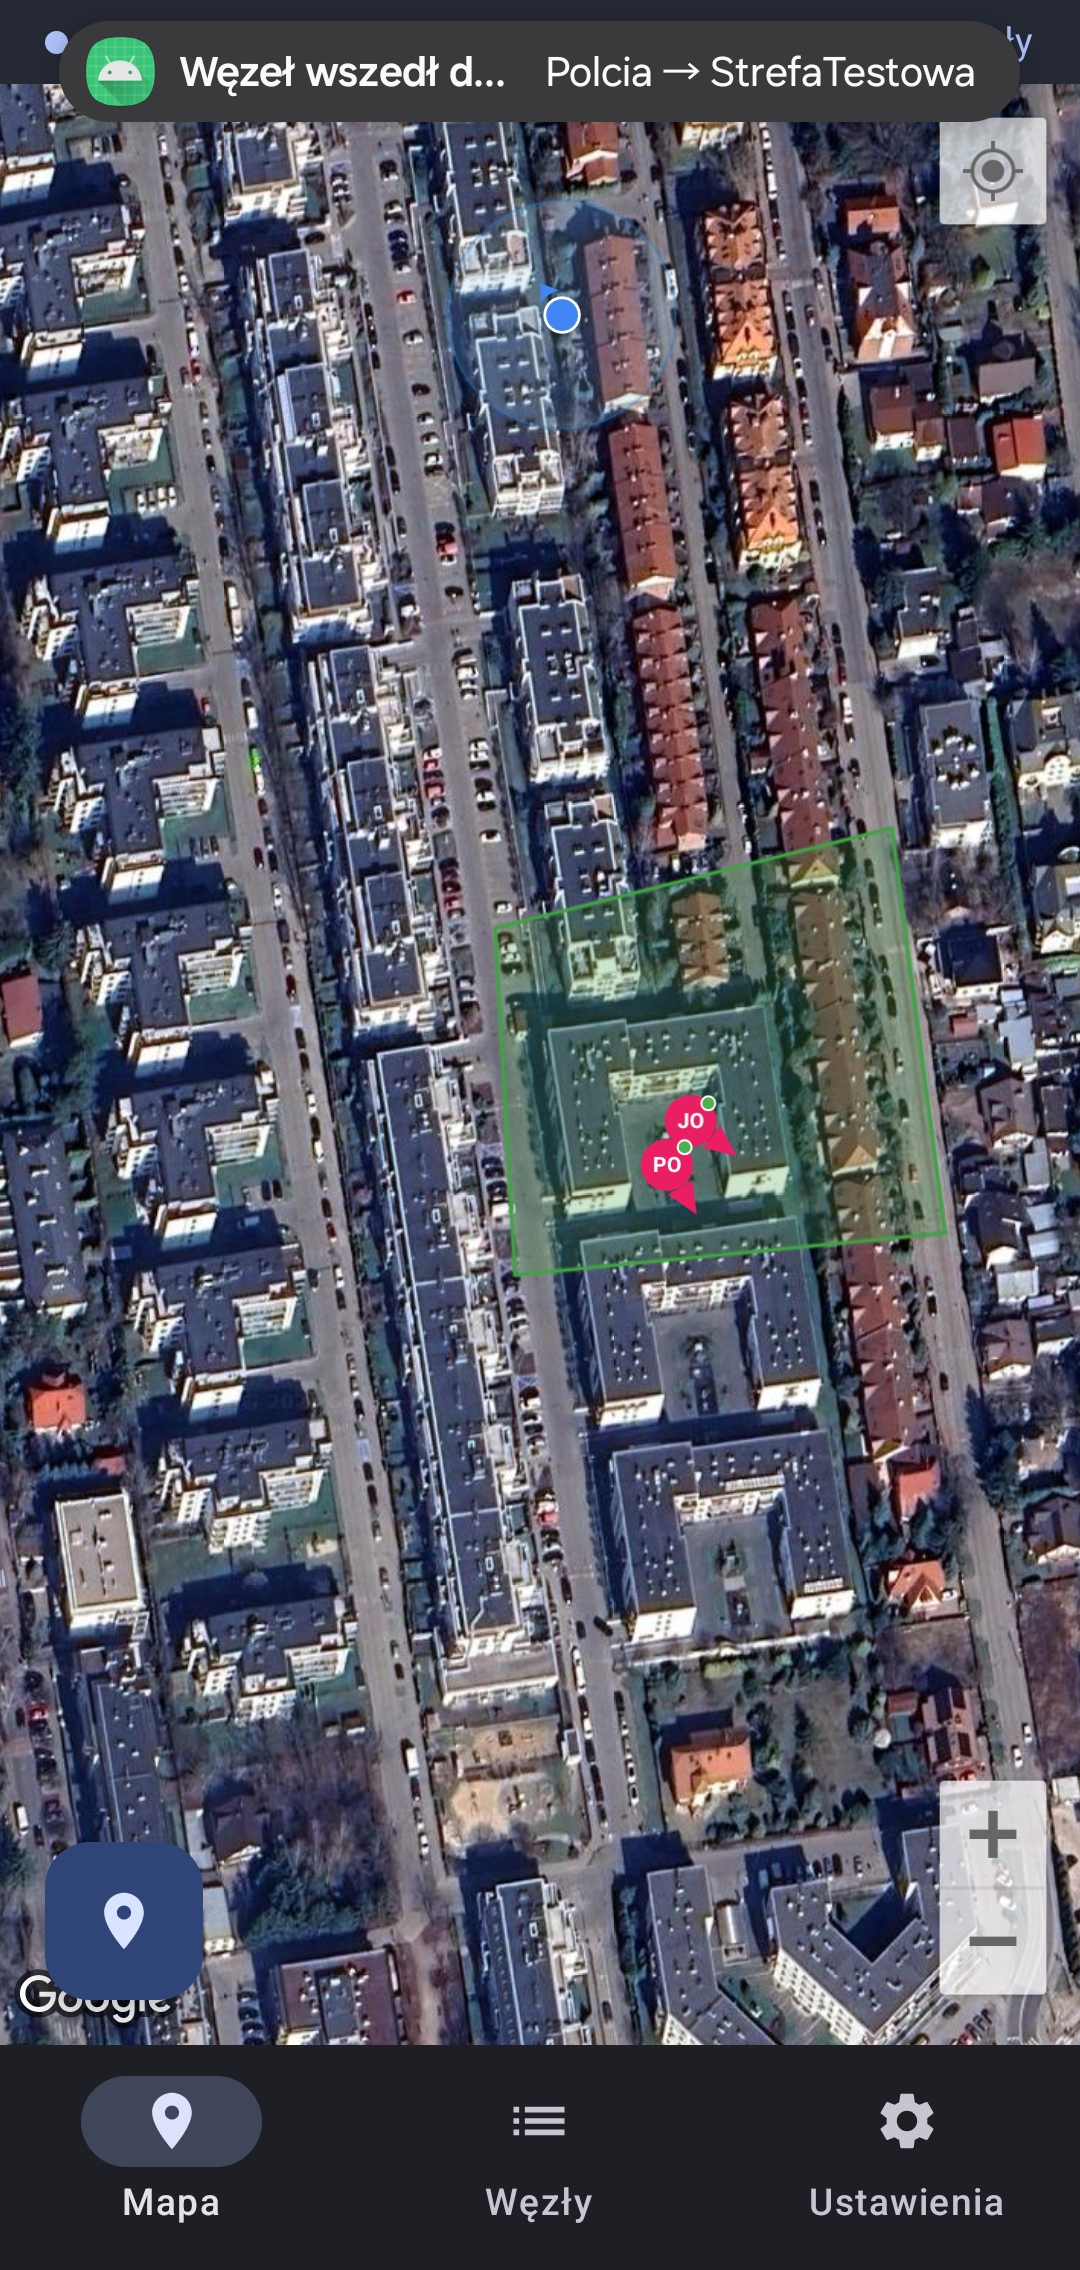
\includegraphics[width=\linewidth]{strefaPowiadomienieWejscia.jpg}
        \caption{Powiadomienie o wejściu w strefę}
        \label{fig:strefa-powiadomienie-wejscia}
    \end{minipage}
\end{figure}

Dotknięcie powiadomienia otwiera aplikację MeshTracker na ekranie mapy.

\paragraph{Uzasadnienie wyboru i metody alternatywne.}

Przed wyborem ray castingu rozważono kilka innych podejść, które warto
tu opisać - zarówno dlatego, że ich odrzucenie było nieoczywiste, jak i dlatego, że
w innych scenariuszach mogłyby być lepszym wyborem.

\textbf{Strefa okrągła (promień od centrum).}
Pierwszym pomysłem była strefa jako okrąg o środku $C = (x_C, y_C)$
i promieniu $r$. Sprawdzenie przynależności sprowadza się wtedy do prostego porównania:
\[
    d(P, C) \leq r \;\Leftrightarrow\; \text{punkt wewnątrz strefy}
\]
To rozwiązanie jest szybsze obliczeniowo i prostsze w implementacji, ponieważ nie trzeba
przechowywać listy wierzchołków. Rozwiązanie to odrzucono, ze względu na elastyczność. 
Zazwyczaj działki mają kształty zbliżone do wydłużonego wielokąta, a nie koła. 
Okrąg wystarczająco duży, żeby objąć cały teren, wychodziłby daleko poza drogę przy granicy działki, przez co alarm byłby
spóźniony. Okrąg wystarczająco mały, żeby nie wychodzić za drogę, nie obejmowałby
części terenu. Wielokąt pozwala narysować granicę dokładnie wzdłuż ogrodzenia sąsiada,
polnej miedzy, albo linii lasu.

\textbf{Google Geofencing API.}
Wstępnie rozważano skorzystanie z gotowego
geofencing API, które Android udostępnia właśnie do monitorowania przekroczeń granic
geograficznych. Szybko okazało się jednak, że to API monitoruje wyłącznie pozycję GPS
\emph{samego telefonu} i obsługuje tylko strefy okrągłe.


\textbf{Algorytm liczby owiniętej (ang.\ \textit{winding number}).}
W literaturze dotyczącej problemu PIP ~\cite{shimrat1962} zidentyfikowano również ten algorytm, który zlicza,
ile razy wielokąt owija się wokół badanego punktu. Jest numerycznie bardziej stabilny od
ray castingu, tzn.\ lepiej obsługuje przypadki brzegowe, gdzie punkt leży dokładnie na krawędzi
wielokąta. W kontekście niniejszego projektu rozróżnienie to jest jednak akademickie: Przy dokładności GPS rzędu kilku metrów prawdopodobieństwo, że zmierzony punkt
znajdzie się dokładnie na krawędzi wielokąta zdefiniowanego przez użytkownika, jest
pomijalnie małe. Wybór padł na ray casting, ponieważ implementacja jest krótsza, prostsza do zrozumienia
i wystarczająca na potrzeby projektu. Złożoność obliczeniowa obu algorytmów wynosi $O(n)$.

\textbf{Indeksowanie przestrzenne (R-tree\footnote{R-tree - hierarchiczna struktura danych do indeksowania obiektów przestrzennych, grupująca je w zagnieżdżone prostokąty otaczające. Umożliwia szybkie wyszukiwanie przestrzenne w czasie $O(\log n)$.}).}
W przypadku konieczności obsługiwania setek stref jednocześnie, sprawdzanie każdej z nich przy 
aktualizacji pozycji stanowiłoby istotne ograniczenie wydajności.
Struktury takie jak R-tree pozwalają szybko zawęzić kandydatów do stref, których obwiednia
prostokątna zawiera dany punkt. W MeshTrackerze spodziewanych jest co najwyżej kilka stref
i kilka węzłów - indeksowanie nie przyniosłoby żadnych mierzalnych korzyści, a znacznie
skomplikowałoby implementację.

\section{Przechowywanie i eksport historii pozycji}
\label{sec:historia-eksport}

Aby umożliwić analizę zebranych danych pomiarowych, konieczne było zaimplementowanie mechanizmu
przechowywania historii pozycji węzłów oraz funkcji eksportu tych danych do formatu CSV.
Zaimplementowano cztery funkcjonalności: 
- mechanizm przechowywania historii pozycji węzłów i wyświetlania "śladu" na mapie
- eksport zebranych danych pozycji do pliku CSV, 
- eksport logu zdarzeń geofencingu (wejść i wyjść ze stref) 
- eksport definicji stref (geometrii wielokątów wraz z listą obserwowanych węzłów). 
Pierwsze dwie funkcjonalności mogą służyć użytkownikowi do wizualizacji ścieżki, którą poruszał się węzeł. Kolejne dwie funkcjonalności potrzebne są w większym stopniu do sprawdzenia dokładności, a co za tym idzie "przydatności" aplikacji i systemu. Eksport definicji stref umożliwia odtworzenie geometrii stref poza aplikacją - np. do naniesienia na mapę i obliczenia odległości wystąpienia zdarzenia WEJŚCIA/WYJŚCIA do/ze strefy od rzeczywistego miejsca przecięcia granicy strefy i ścieżki węzła. 

\subsection*{Przechowywanie historii pozycji}
\label{sec:historia}

\paragraph{Model danych.}

Pojedynczy punkt reprezentuje klasa \texttt{TimedPosition}:

\begin{lstlisting}[caption={Klasa \texttt{TimedPosition} - pojedynczy punkt},
                   label={lst:timed-position}]
data class TimedPosition(
    val latitude: Double,
    val longitude: Double,
    val altitude: Int,
    val timestampSeconds: Int,
    val snr: Float
    val rssi: Int
)
\end{lstlisting}

Stan przechowywany jest wyłącznie w~pamięci operacyjnej, dlatego restart aplikacji
powoduje utratę historii - jest to zachowanie celowe, ponieważ dane sesji pomiarowej
nie powinny wpływać na kolejne sesje.

\subsection*{Eksport danych sesji do CSV}
\label{sec:eksport-csv}

Eksportem zajmuje się \texttt{CsvExporter}, który zbiera dane z~\texttt{\seqsplit{PositionHistoryRepository}}
i~\texttt{\seqsplit{PacketStatsRepository}}, a~następnie zapisuje plik przez standardowy mechanizm \texttt{MediaStore.Downloads}. Nagłówek zawiera 16 kolumn zebranych w (tabli~\ref{tab:csv-kolumny}).

\begin{table}[!h]
    \caption{Kolumny pliku CSV}
    \label{tab:csv-kolumny}
    \centering
    \small
    \begin{tabular}{|p{3.2cm}|p{4.3cm}|p{5.5cm}|}
        \hline
        \textbf{Kolumna} & \textbf{Źródło} & \textbf{Uwagi} \\
        \hline
        \texttt{timestamp\_unix}    & \texttt{\seqsplit{TimedPosition.timestampSeconds}} & Czas GPS lub czas odbioru \\
        \texttt{\seqsplit{timestamp\_readable}}& j.w., sformatowany & \texttt{yyyy-MM-dd HH:mm:ss} \\
        \texttt{node\_id}           & \texttt{\seqsplit{MeshNodeInfo.getId()}} & np.\ \texttt{!a1b2c3d4} \\
        \texttt{node\_name}         & \texttt{\seqsplit{MeshNodeInfo.getDisplayName()}} & Snapshot z~chwili eksportu \\
        \texttt{role}               & \texttt{MeshUser.role} & CLIENT, TRACKER, ROUTER itd. \\
        \texttt{lat}, \texttt{lng}  & \texttt{TimedPosition} & 6 miejsc po przecinku \\
        \texttt{altitude\_m}        & \texttt{\seqsplit{TimedPosition.altitude}} &  \\
        \texttt{snr\_db}            & \texttt{MeshNodeInfo.snr} & Puste jeśli \texttt{Float.MAX\_VALUE} \\
        \texttt{rssi\_dbm}          & \texttt{MeshNodeInfo.rssi} & Puste jeśli \texttt{Int.MAX\_VALUE} \\
        \texttt{delta\_t\_s}        & \texttt{PacketStatsRepository} & $\Delta t$ od poprzedniego broadcastu \\
        \hline
    \end{tabular}
    \normalsize
\end{table}

Każdy punkt z~historii \texttt{PositionHistoryRepository} staje się jednym wierszem CSV.
Węzły bez historii pozycji (np.\ węzły wewnątrz budynku, bez fixa GPS) eksportowane są
jako jeden wiersz z~aktualnym stanem - kolumny \texttt{lat} i~\texttt{lng} pozostają
puste, natomiast dostępne metadane (SNR, RSSI, bateria) są wypełniane.

Jeśli historia jest pusta, metoda zwraca \texttt{Result.failure} z~komunikatem
\texttt{"empty"} i~plik nie jest tworzony.

\paragraph{Interfejs użytkownika.}

Eksport całej sesji dostępny jest w~sekcji ,,Dane testowe'' ekranu ustawień
(rysunek~\ref{fig:ustawienia-eksport}). Przycisk ,,Eksportuj sesję do CSV'' wywołuje
\texttt{\seqsplit{SettingsViewModel.exportSession()}}, który uruchamia \texttt{CsvExporter.export()}.
Po zakończeniu otwiera Android Share sheet z~gotowym plikiem. Przycisk ,,Wyczyść historię pozycji''
wywołuje \texttt{\seqsplit{positionHistoryRepository.clearAll()}} oraz
\texttt{\seqsplit{packetStatsRepository.resetAll()}} po potwierdzeniu przez \texttt{AlertDialog}.

\begin{figure}[h]
    \centering
    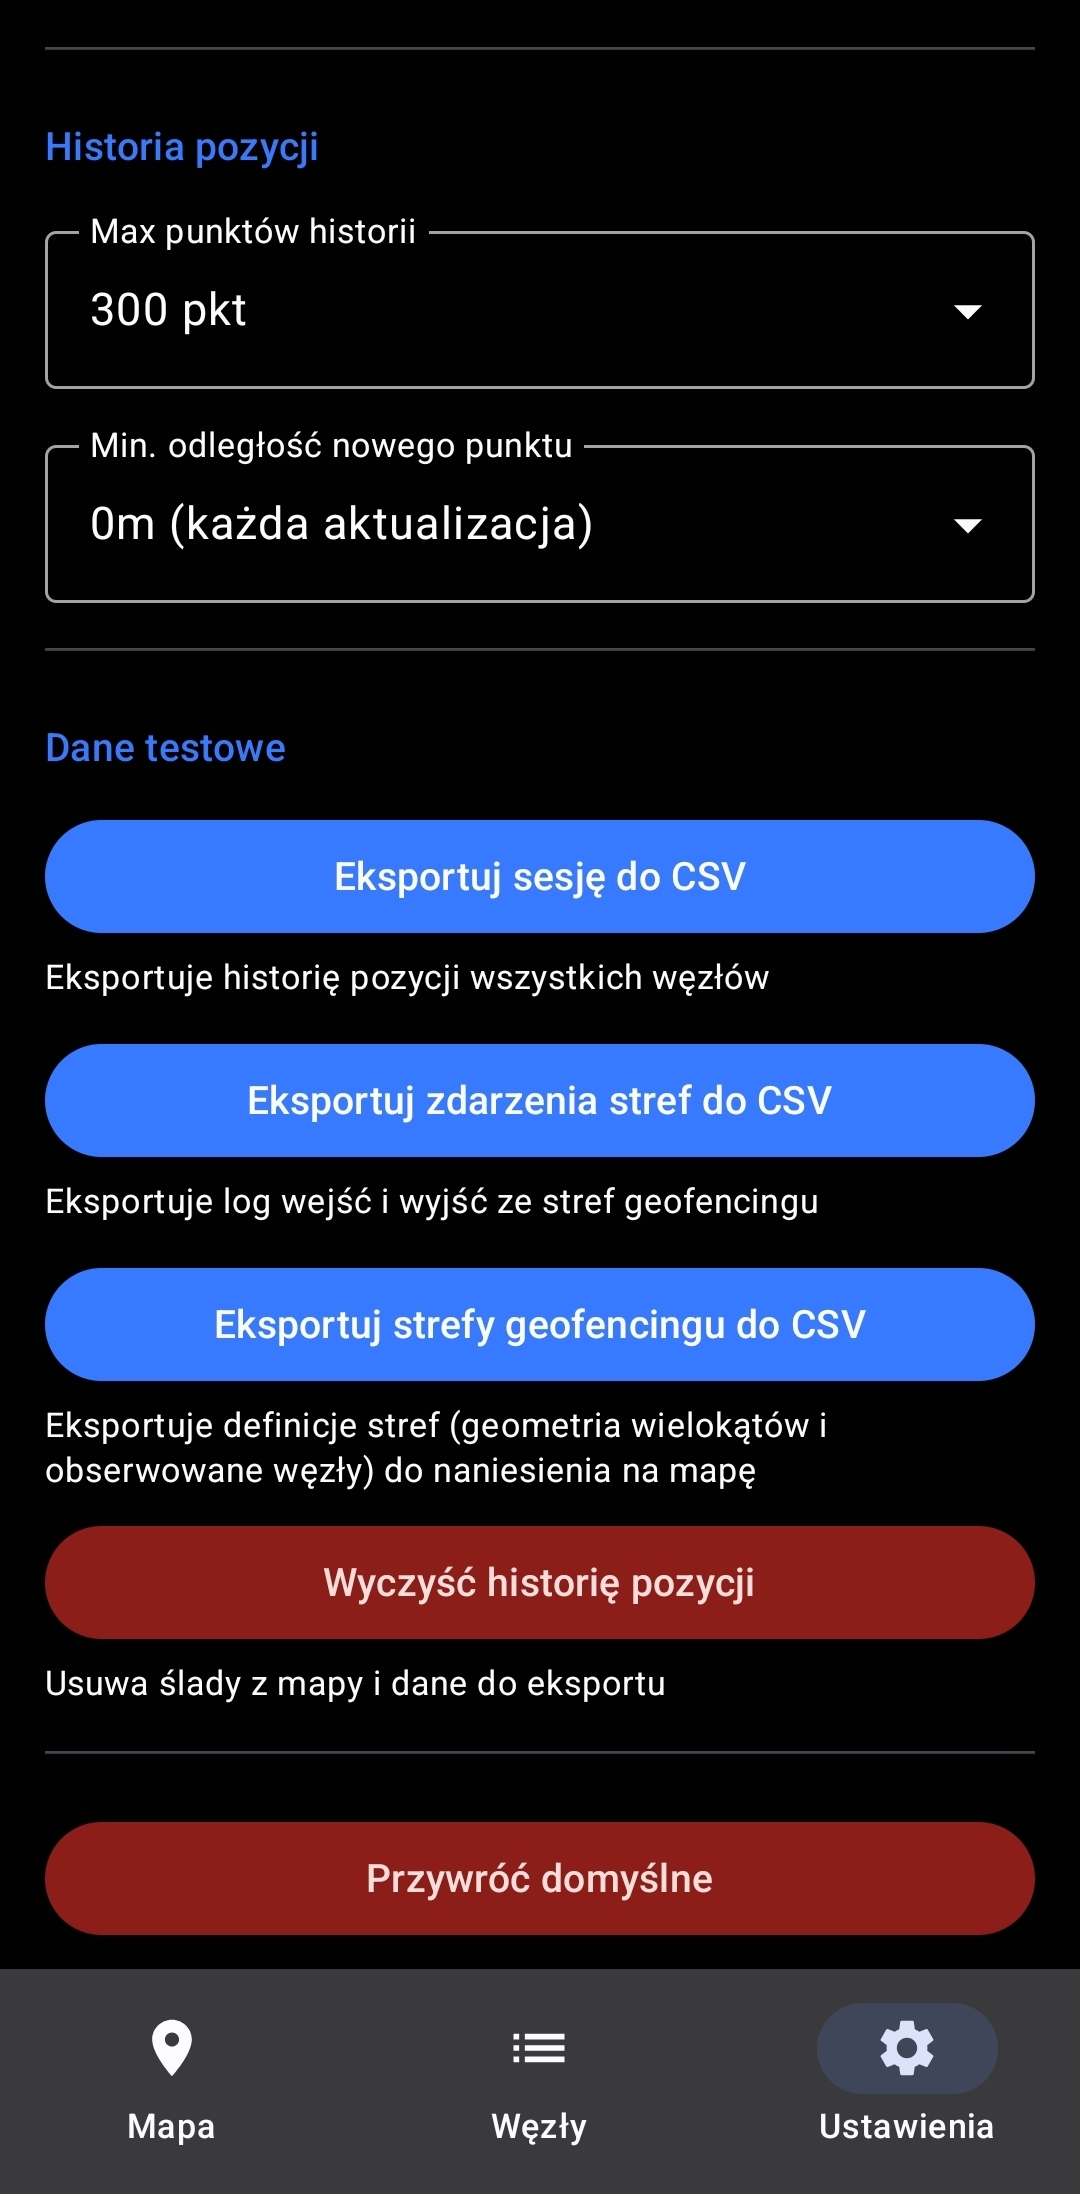
\includegraphics[width=0.45\linewidth]{img/ustawieniaEksport.jpg}
    \caption{Sekcja ,,Dane testowe'' w~ekranie ustawień aplikacji}
    \label{fig:ustawienia-eksport}
\end{figure}

\subsection*{Eksport zdarzeń geofencingu do CSV}
\label{sec:eksport-strefy}

Zdarzenia wejść i~wyjść ze stref (encja \texttt{ZoneEvent}, omówiona
w~rozdz.~\ref{sec:geofencing}) są przechowywane w~bazie Room i~nie są tracone po
restarcie aplikacji. Umożliwia to eksport pełnego logu zdarzeń z~całej sesji terenowej, nawet jeśli aplikacja była w~międzyczasie restartowana. Nazwa pliku przyjmuje format 
\texttt{meshtracker\_zones\_YYYYMMDD\_HHmmss.csv}, a plik zawiera 7 kolumn wymienionych w 

\begin{table}[!h]
    \caption{Kolumny pliku CSV zdarzeń stref}
    \label{tab:csv-strefy}
    \centering
    \small
    \begin{tabular}{|p{3.2cm}|p{4cm}|p{5cm}|}
        \hline
        \textbf{Kolumna} & \textbf{Źródło} & \textbf{Uwagi} \\
        \hline
        \texttt{timestamp\_unix}    & \texttt{\seqsplit{ZoneEvent.timestampSeconds}} & Czas rejestracji zdarzenia przez telefon \\
        \texttt{\seqsplit{timestamp\_readable}}& j.w., sformatowany & \texttt{yyyy-MM-dd HH:mm:ss} \\
        \texttt{zone\_id}           & \texttt{ZoneEvent.zoneId}           & UUID strefy \\
        \texttt{zone\_name}         & \texttt{Zone.name}                  & Nazwa nadana przez użytkownika \\
        \texttt{node\_id}           & \texttt{ZoneEvent.nodeId}           & Identyfikator węzła \\
        \texttt{node\_name}         & \texttt{\seqsplit{ZoneEvent.nodeName}}         & Snapshot nazwy z~chwili zdarzenia \\
        \texttt{event\_type}        & \texttt{\seqsplit{ZoneEvent.eventType}}        & \texttt{ENTER} lub \texttt{EXIT} \\
        \hline
    \end{tabular}
    \normalsize
\end{table}

Wiersze posortowane są rosnąco według znacznika czasu, co ułatwia obliczenie czasu
$T_z$ jako różnicy między fizycznym przekroczeniem granicy a~timestampem wiersza
\texttt{ENTER} lub \texttt{EXIT} w~arkuszu kalkulacyjnym.

\paragraph{Implementacja.}

Metoda \texttt{\seqsplit{CsvExporter.exportZoneEvents()}} pobiera zdarzenia ze wszystkich stref  -
zarówno aktywnych, jak i~dezaktywowanych  - ponieważ log historyczny nie powinien
zależeć od bieżącej konfiguracji monitoringu. Dostęp do bazy odbywa się przez dwa
jednorazowe zapytania DAO (\texttt{\seqsplit{getAllZonesOnce()}}, \texttt{\seqsplit{getEventsOnce(zoneId)}}),
a nie przez \texttt{Flow}, co jest właściwe w~kontekście \texttt{Dispatchers.IO}.

\paragraph{Interfejs użytkownika.}

W~sekcji ,,Dane testowe'' ekranu ustawień, poniżej przycisku ,,Eksportuj sesję do CSV'',
znajduje się przycisk ,,Eksportuj zdarzenia stref do CSV''. Wywołuje on
\texttt{\seqsplit{SettingsViewModel.exportZoneEvents()}}, a~wynik trafia do osobnego kanału
\texttt{\seqsplit{exportZonesEvent}}, obsługiwanego przez dedykowany \texttt{\seqsplit{LaunchedEffect}}
w~\texttt{SettingsScreen}. Jeśli baza nie zawiera żadnych zdarzeń, plik nie jest tworzony.

\subsection*{Eksport definicji stref geofencingu do CSV}
\label{sec:eksport-definicje-stref}

Trzeci wariant eksportu dotyczy samej \textbf{konfiguracji} stref -
geometrii wielokątów i~listy węzłów, które dana strefa monitoruje
tabela~\ref{tab:zone-entity}). W~odróżnieniu od eksportu zdarzeń (rozdz.~\ref{sec:eksport-strefy}),
który dokumentuje \emph{co się wydarzyło}, ten eksport dokumentuje \emph{jak zdefiniowano
strefę} - pozwala to np.\ odtworzyć granice stref w~zewnętrznym narzędziu GIS albo zachować
kopię zapasową konfiguracji przed jej modyfikacją lub usunięciem. Nazwa pliku przyjmuje format\\
\texttt{meshtracker\_zone\_definitions\_YYYYMMDD\_HHmmss.csv}.
Plik zawiera 8 kolumn (tabela~\ref{tab:csv-definicje-stref})

\begin{table}[!h]
    \caption{Kolumny pliku CSV definicji stref}
    \label{tab:csv-definicje-stref}
    \centering
    \small
    \begin{tabular}{|p{3cm}|p{3.7cm}|p{5.3cm}|}
        \hline
        \textbf{Kolumna} & \textbf{Źródło} & \textbf{Uwagi} \\
        \hline
        \texttt{zone\_id}            & \texttt{Zone.id}                          & UUID strefy \\
        \texttt{zone\_name}          & \texttt{Zone.name}                        & Nazwa nadana przez użytkownika \\
        \texttt{color\_argb}         & \texttt{\seqsplit{Zone.colorArgb}}        & Kolor strefy jako liczba ARGB \\
        \texttt{is\_active}          & \texttt{\seqsplit{Zone.isActive}}         & \texttt{true}/\texttt{false} \\
        \texttt{vertex\_index}       & Indeks w~liście wierzchołków              & Numeracja od 0 \\
        \texttt{vertex\_lat}, \texttt{vertex\_lon} & \texttt{\seqsplit{Zone.vertices()}} & 6 miejsc po przecinku \\
        \texttt{watched\_node\_ids}  & \texttt{\seqsplit{Zone.watchedNodeIds()}} & Lista ID węzłów rozdzielona średnikiem \texttt{;} \\
        \hline
    \end{tabular}
    \normalsize
\end{table}

Każdy wierzchołek wielokąta strefy staje się jednym wierszem CSV - dzięki temu plik
zachowuje pełną geometrię, kosztem denormalizacji (kolumny \texttt{zone\_id} .. \texttt{is\_active}
oraz \texttt{watched\_node\_ids} powtarzają się w~każdym wierszu należącym do tej samej
strefy). Jeżeli strefa nie posiada żadnych wierzchołków (przypadek brzegowy), eksportowany
jest pojedynczy wiersz z~pustymi kolumnami \texttt{vertex\_index}, \texttt{vertex\_lat}
i~\texttt{vertex\_lon}.

\paragraph{Implementacja.}

Metoda \texttt{\seqsplit{CsvExporter.exportZoneDefinitions()}} pobiera wszystkie strefy przez
\texttt{\seqsplit{zoneRepository.getAllZonesOnce()}} - zarówno aktywne, jak i~nieaktywne - a~następnie
dla każdej z~nich generuje wiersze na podstawie jej wierzchołków. Jeśli w~bazie nie ma
żadnej zdefiniowanej strefy, metoda zwraca \texttt{Result.failure} z~komunikatem
\texttt{"empty"} i~plik nie jest tworzony.

\paragraph{Interfejs użytkownika.}

W~sekcji ,,Dane testowe'' ekranu ustawień, poniżej przycisku ,,Eksportuj zdarzenia stref
do CSV'', znajduje się trzeci przycisk - ,,Eksportuj strefy geofencingu do CSV'', opisany
podpisem ,,Eksportuje definicje stref (geometria wielokątów i~obserwowane węzły) do
naniesienia na mapę'' (rysunek~\ref{fig:ustawienia-eksport}). Wywołuje on
\texttt{\seqsplit{SettingsViewModel.exportZoneDefinitions()}}, a~wynik trafia do osobnego
kanału \texttt{\seqsplit{exportZoneDefinitionsEvent}}, obsługiwanego przez dedykowany
\texttt{\seqsplit{LaunchedEffect}} w~\texttt{SettingsScreen}, który otwiera Android Share
sheet z~tytułem ,,Eksportuj strefy geofencingu''.

\newpage
\section{Zakończenie}
\label{sec:zakonczenie}

\subsection*{Podsumowanie realizacji celu pracy}

Celem pracy, sformułowanym w~rozdz.~\ref{sec:wstep}, było zaprojektowanie i~implementacja systemu
monitorowania położenia zwierząt w~czasie rzeczywistym, działającego w~obszarach pozbawionych
pokrycia sieci komórkowej, wraz z~aplikacją mobilną umożliwiającą wizualizację położenia na mapie,
definiowanie wirtualnych stref bezpieczeństwa oraz powiadamianie użytkownika o~ich przekroczeniu.

Cel ten został zrealizowany. Rozdz.~\ref{sec:wymagania} przełożył motywację (ucieczki psa myśliwskiego
poza teren pozbawiony ogrodzenia i~zasięgu sieci komórkowej) na trzy konkretne problemy inżynierskie -
transmisję danych bez infrastruktury zewnętrznej, optymalizację zajętości pasma oraz integrację
aplikacji mobilnej z~siecią radiową - a~także na mierzalne wymagania funkcjonalne i~parametryczne.
Rozdz.~\ref{sec:modulacja-lora} opisuje dobór technologii LoRa/Meshtastic i~konfigurację sprzętu
radiowego rozwiązujący problem pierwszy, rozdz.~\ref{sec:integracja-meshtastic} - integrację aplikacji
mobilnej z~siecią radiową (problem trzeci), a~rozdz.~\ref{sec:geofencing} - mechanizm geofencingu
oparty na algorytmie ray casting wraz z~modelem stref i~zdarzeń. Rozdz.~\ref{sec:podsumowanie-testy}
potwierdza w~oparciu o~testy terenowe, że zbudowany system poprawnie wykrywa przekroczenie granicy
strefy zarówno w~typowych, jak i~skrajnych warunkach.

Problem drugi - optymalizacja zajętości pasma poprzez adaptacyjną częstotliwość wysyłania pozycji
zależną od stanu ruchu węzła - pozostaje częściowo otwarty; w~przeprowadzonych testach system
korzystał ze stałego interwału próbkowania GPS (5~s) narzuconego przez firmware Meshtastic
(por.\ rozdz.~\ref{sec:podsumowanie-testy}), a~nie z~mechanizmu adaptacyjnego. Kwestię tę rozwinięto
w~rozdziale ,,Możliwości dalszego rozwoju''.

\subsection*{Wnioski z~oceny rozwiązania}

Zestawienie z~komercyjnymi systemami śledzenia psów myśliwskich (tab.~\ref{tab:porownanie}) oraz
wyniki testów terenowych (rozdz.~\ref{sec:podsumowanie-testy}) pozwalają sformułować następujące
wnioski.

Architektura mesh nie ogranicza zasięgu systemu do pojedynczego łącza
nadajnik-odbiornik, jak w~rozwiązaniach Dogtra i~Dogtrace, lecz pozwala go rozszerzać przez
dodawanie kolejnych węzłów pośredniczących - potwierdzają to testy zasięgu
(tab.~\ref{tab:zasieg-efektywny}), w~których dodanie trzeciego węzła zwiększyło zasięg efektywny
z~2052~m do 2278~m. System zbudowany jest z~ogólnodostępnych komponentów za ok.\ 400~PLN za węzeł,
czyli znacząco taniej niż rozwiązania komercyjne (2500~PLN i~2300~PLN), przy jednoczesnym braku
sztywnego limitu liczby węzłów (21 dla Dogtra, 19 dla Dogtrace). Testy precyzji geofencingu
(rozdz.~\ref{sec:precyzja-geofencingu}) wykazały, że wprowadzenie bufora rzędu 6-8~m redukuje
liczbę fałszywych alarmów o~99,6\%, co czyni system praktycznie użytecznym mimo ograniczeń
interwału próbkowania GPS.

Niestety system ma też swoje ogranicznia. Osiągnięty zasięg efektywny (889-2278~m, zależnie od konfiguracji
sprzętowej) jest o~rząd wielkości mniejszy niż w~systemach komercyjnych (14-20~km) - należy jednak
podkreślić, że są to wartości nieporównywalne wprost, ponieważ zasięg systemu mesh rośnie wraz
z~liczbą węzłów pośredniczących, a~zasięg systemów punkt-punkt jest stały. Dodatkowo deklarowane przez producentów
marketingowe metryki często nie w znacznej mierze nie pokrywają się z rzeczywistymi wartościami. Co istotne, konfiguracja
bazowa oparta wyłącznie na węzłach T-1000-E (889~m) \emph{nie spełnia} przyjętego w~rozdz.~\ref{sec:wymagania}
wymagania minimalnego zasięgu 2~km - wymaganie to jest spełnione dopiero po zastosowaniu węzła
T-Beam po stronie bazy (2052~m) lub dodaniu przekaźnika (2278~m). Błąd zgłoszenia przekroczenia
granicy strefy jest w~praktyce zdominowany przez interwał próbkowania GPS (5~s), a~nie przez
niedoskonałości algorytmu ray casting - jest to ograniczenie po stornie sprzętu i protokołu (firmware
Meshtastic), a~nie implementacyjne. Jako ostatnie ogranicznie trzeba zwrócić uwagę na to, że ochrona 
obudowy węzła mobilnego (IP65) jest niższa niż w~rozwiązaniach komercyjnych (IPX9K, IP68).

\subsection*{Zakres zastosowań i~perspektywy wdrożenia}

Choć bezpośrednim punktem wyjścia było śledzenie psa myśliwskiego, opracowane rozwiązanie -
sieć mesh LoRa z~aplikacją mobilną obsługującą geofencing dowolnych wielokątów - nie jest
specyficzne dla tego jednego zastosowania. Ten sam mechanizm mógłby posłużyć do monitorowania
zwierząt gospodarskich na dużych, otwartych pastwiskach pozbawionych zasięgu sieci komórkowej,
innych zwierząt domowych, a~także - po odpowiednich modyfikacjach interfejsu - do pilnowania mienia
lub sprzętu pozostawionego w~terenie (analogicznie do funkcji WAYPOINT/FENCE oferowanych przez
Dogtrace, tab.~\ref{tab:porownanie}).

Przed wdrożeniem produkcyjnym system wymagałby jednak dodatkowej walidacji, wykraczającej poza
zakres niniejszej pracy:
\begin{itemize}
    \item pomiaru rzeczywistego czasu pracy węzła mobilnego na baterii w~warunkach terenowych
          (aspekt ten nie był przedmiotem testów opisanych w~rozdz.~\ref{sec:podsumowanie-testy}),
    \item testów z~większą liczbą jednocześnie monitorowanych zwierząt/węzłów niż trzy użyte
          w~testach zasięgu,
    \item potwierdzenia szczelności obudowy w~warunkach długotrwałej ekspozycji (deszcz, błoto,
          zanurzenie częściowe) wykraczających poza deklarację IP65,
    \item oszacowania kosztu produkcji seryjnej (obecna wycena ok.\ 400~PLN/węzeł dotyczy
          pojedynczych egzemplarzy, por.\ tab.~\ref{tab:porownanie}).
\end{itemize}

\newpage
\subsection*{Możliwości dalszego rozwoju}

Na podstawie zidentyfikowanych ograniczeń można wskazać kilka kierunków dalszego rozwoju systemu.
Szczególnie istotne wydaje się zrealizowanie adaptacyjnej częstotliwości wysyłania pozycji,
zależnej od stanu ruchu węzła - a więc rzadszego próbkowania podczas bezruchu i~częstszego
w~pobliżu granicy strefy - co pozwoliłoby wypełnić wymaganie sformułowane w~rozdz.~\ref{sec:wymagania},
dotychczas niezrealizowane wobec stałego interwału próbkowania GPS narzuconego przez firmware
Meshtastic. Poza oczywistą korzyścią w~postaci oszczędności baterii węzła mobilnego, rozwiązanie
to miałoby również bezpośredni wpływ na jakość działania systemu: skrócenie efektywnego interwału
próbkowania w~otoczeniu granicy strefy powinno zmniejszyć błąd zgłoszenia przekroczenia opisany
w~rozdz.~\ref{sec:precyzja-geofencingu}, bez konieczności utrzymywania wysokiej częstotliwości
próbkowania - a~więc i~zwiększonego zużycia energii oraz pasma - na całym obszarze monitorowanym.
Kolejnym kierunkiem wartym zbadania jest współpraca z~dronem, wykorzystanym w~niniejszej
pracy dotychczas jedynie jako narzędzie testowe do odtwarzania powtarzalnej trasy węzła mobilnego.
Docelowo dron mógłby pełnić funkcję aktywnego elementu systemu - unoszący się nad terenem węzeł, 
dzięki wyniesieniu ponad przeszkody terenowe, mógłby zwiększać zasięg poszukiwań zagubionego 
zwierzęcia oraz poprawiać parametry transmisji (mniejsze tłumienie sygnału, większą niezawodność łącza)
względem konfiguracji opartej wyłącznie na stacjonarnej lub noszonej stacji bazowej.

Dodatkowych badań wymagałyby również testy skalowalności sieci przy liczbie węzłów większej niż
trzy, w~tym analiza zajętości współdzielonego kanału radiowego, sygnalizowana już w~tab.~\ref{tab:porownanie}
(przypis dotyczący nieograniczonej liczby węzłów), a~także pomiar i~optymalizacja czasu pracy na
baterii węzła mobilnego wraz z~doborem trybów oszczędzania energii w~zależności od aktywności
zwierzęcia. Możliwe byłoby wreszcie rozszerzenie aplikacji mobilnej o~analitykę historycznych tras,
wykraczającą poza obecny eksport CSV opisany w~rozdz.~\ref{sec:historia-eksport}, oraz o~wersję
na system iOS.

Z powyższych kierunków szerzej przyjrzymy się pierwszemu, ponieważ miałby on realnie największy wpływ na użytkowanie.
Jak wynika z otwartego kodu firmware'u Meshtastic~\cite{meshtasticFirmwareRepo} oraz opisu API
modułów~\cite{meshtasticModuleApiDocs}, częstotliwością raportowania pozycji sterują dwa oddzielne ustawienia. Jedno ustala, jak często moduł GPS
w~ogóle próbuje złapać nowy namiar, a drugie jak często węzeł nadaje posiadaną pozycję do sieci.
Domyślnie są to odpowiednio 2~minuty i~godzina - w~tej pracy oba skrócono do 5~s, żeby uzyskać
,,gęstszy'' strumień pozycji.

Firmware ma też wbudowany, domyślnie włączony mechanizm ,,inteligentnego'' raportowania: węzeł
nadaje pozycję od razu, gdy przesunie się o~więcej niż jakieś 100~metrów, zamiast czekać na koniec
stałego interwału. To dokładnie ten rodzaj mechanizmu - reagującego na ruch węzła, a~nie na zegar -
był potrzebny do pełnej realizacji ,,problemu drugiego''. Z~kodu wynika jednak, że odstęp między
takimi nadaniami i~tak nie może zejść poniżej 5~minut, niezależnie od tego, co ustawi użytkownik -
to twardy limit wpisany w~firmware. W~praktyce ten wbudowany mechanizm okazuje się więc wolniejszy
niż zwykły, stały interwał 5-sekundowy zastosowany w~pracy i~sam z~siebie nie rozwiązuje problemu
opóźnienia poniżej 3~sekund.

Dosłowne spełnienie tego wymagania wymagałoby więc czegoś więcej niż zmiany ustawień. Jedną
z~opcji byłoby dynamiczne przeprogramowywanie interwału z~poziomu aplikacji mobilnej - skoro
aplikacja już zna geometrię stref i~bieżącą pozycję węzła, mogłaby skracać interwał raportowania
tylko wtedy, gdy zwierzę zbliża się do granicy, a~rozluźniać go w~pozostałym czasie dla
oszczędności baterii. Głębszym, ale trwalszym rozwiązaniem byłoby napisanie własnego modułu 
firmware'u, który przenosiłby geometrię stref na sam węzeł i~decydował o~częstotliwości nadawania
lokalnie, bez pośrednictwa telefonu. Odbyłoby się to kosztem konieczności utrzymywania własnego forka firmware'u.

    Testy zasięgu przebiegały etapami, w~bardzo różnych warunkach terenowych, zanim ostatecznie
oceniono system w~scenerii zbliżonej do docelowego zastosowania. Pierwsze pomiary wykonano
w~zabudowie wielopiętrowej mieszkalnej (widocznej w~tle części zrzutów ekranu w~rozdz.
,,Przegląd ekranów aplikacji'', np.\ rysunek~\ref{fig:map-screen})
i~wykazały zasięg praktycznie ograniczony do bezpośredniej widoczności między węzłami. Kolejne
testy, przeprowadzone na płaskim, otwartym terenie polnym, dały wynik rzędu 2~km, a~testy
w~terenie górskim - rzędu 10~km. Dla porównania, oficjalne testy zasięgu Meshtastic~\cite{meshtasticRangeTests} dokumentują przypadki nawiązania
łączności na dystansie sięgającym kilkuset kilometrów - trzeba jednak wyraźnie zastrzec, że są to
warunki skrajnie sprzyjające (bezpośrednia widzialność optyczna, znaczna wysokość umieszczenia
anten, sprzyjająca propagacja radiowa), zupełnie niereprezentatywne dla docelowego zastosowania
systemu, czyli obroży psa poruszającego się nisko nad ziemią, w~terenie często zalesionym.

Dopiero testy przeprowadzone w~scenerii najbliższej docelowej tnz. terenie o charakterze rolniczo-leśnym na
Mazurach- pokazały, że efektywny zasięg gwarantujący dostarczenie 90\% pakietów jest znacząco mniejszy niż sugerowałyby wcześniejsze pomiary w~terenie
otwartym czy górskim (889-2278~m, tab.~\ref{tab:zasieg-efektywny}). Zależność zasięgu systemu od
typu terenu okazała się na tyle silna, że wynik uzyskany w~jednych warunkach nie przekładał się
wprost na inne - nie był to wniosek oczywisty na początku realizacji pracy.

Gdybym zaczynał pracę od nowa, zakupiłbym bardziej różnorodny zbiór modułów Meshtastic, o różnych parametrach anten oraz baterii, aby przetestować
różne kombinacje sprzętu w~roli stacji bazowej jeszcze przed ostatecznym wyborem platformy
(rozdz.~\ref{sec:modulacja-lora}), zamiast dopiero w~testach końcowych
(rozdz.~\ref{sec:zasieg-siec}). Pozwoliłoby to ocenić zależność zasięgu od typu anteny i~mocy
nadajnika na wczesnym etapie projektu i~ewentualnie skorygować dobór sprzętu, zanim wybór ten
wpłynął na architekturę całego systemu. 
\newpage
Na zakończenie pracy przedstawiam, często wspominanego w tej pracy, psa rasy Mały Gończy Gaskoński, który był inspiracją dla stworzenia niniejszej pracy oraz
służył do testów w terenie. 

\begin{figure}[!t]
  \centering
    
\includegraphics[width=0.8\linewidth]{WUT-Thesis/img/reja_meshtracker.jpg}
    \caption{Mały gończy Gaskoński}
    \label{fig:piesDoTestow}
\end{figure}


%--------------------------------------------
% Literatura
%--------------------------------------------
\cleardoublepage % Zaczynamy od nieparzystej strony
\printbibliography

%--------------------------------------------
% Spisy
%--------------------------------------------
\newpage
\pagestyle{plain}

\listoffigurestoc     % Spis rysunków.
\vspace{1cm}
\listoftablestoc      % Spis tabel.

\end{document} % Dobranoc.
